%Version 3 December 2023
% See section 11 of the User Manual for version history
%
%%%%%%%%%%%%%%%%%%%%%%%%%%%%%%%%%%%%%%%%%%%%%%%%%%%%%%%%%%%%%%%%%%%%%%
%%                                                                 %%
%% Please do not use \input{...} to include other tex files.       %%
%% Submit your LaTeX manuscript as one .tex document.              %%
%%                                                                 %%
%% All additional figures and files should be attached             %%
%% separately and not embedded in the \TeX\ document itself.       %%
%%                                                                 %%
%%%%%%%%%%%%%%%%%%%%%%%%%%%%%%%%%%%%%%%%%%%%%%%%%%%%%%%%%%%%%%%%%%%%%

%%\documentclass[referee,sn-basic]{sn-jnl}% referee option is meant for double line spacing

%%=======================================================%%
%% to print line numbers in the margin use lineno option %%
%%=======================================================%%

% \documentclass[lineno,sn-basic]{sn-jnl}% Basic Springer Nature Reference Style/Chemistry Reference Style

%%======================================================%%
%% to compile with pdflatex/xelatex use pdflatex option %%
%%======================================================%%

%%\documentclass[pdflatex,sn-basic]{sn-jnl}% Basic Springer Nature Reference Style/Chemistry Reference Style


%%Note: the following reference styles support Namedate and Numbered referencing. By default the style follows the most common style. To switch between the options you can add or remove “Numbered” in the optional parenthesis. 
%%The option is available for: sn-basic.bst, sn-vancouver.bst, sn-chicago.bst%  
 
%%\documentclass[pdflatex,sn-nature]{sn-jnl}% Style for submissions to Nature Portfolio journals
%%\documentclass[pdflatex,sn-basic]{sn-jnl}% Basic Springer Nature Reference Style/Chemistry Reference Style
%\documentclass[pdflatex,sn-mathphys-num]{sn-jnl}% Math and Physical Sciences Numbered Reference Style 
%\documentclass[pdflatex,sn-mathphys-ay]{sn-jnl}% Math and Physical Sciences Author Year Reference Style
%%\documentclass[pdflatex,sn-aps]{sn-jnl}% American Physical Society (APS) Reference Style
%%\documentclass[pdflatex,sn-vancouver,Numbered]{sn-jnl}% Vancouver Reference Style
%%\documentclass[pdflatex,sn-apa]{sn-jnl}% APA Reference Style 
\documentclass[pdflatex,sn-chicago]{sn-jnl}% Chicago-based Humanities Reference Style

%%%% Standard Packages
%%<additional latex packages if required can be included here>

\usepackage{graphicx}%
\usepackage{multirow}%
\usepackage{amsmath,amssymb,amsfonts}%
\usepackage{amsthm}%
\usepackage{lmodern}  % Scalable fonts for better support across sizes
\usepackage{mathrsfs}  % Since you're already using this for mathematical symbols
\usepackage[title]{appendix}%
\usepackage{xcolor}%
\usepackage{textcomp}%
\usepackage{manyfoot}%
\usepackage{booktabs}%
\usepackage{algorithm}%
\usepackage{algorithmicx}%
\usepackage{algpseudocode}%
\usepackage{listings}%
\usepackage{lmodern}  % For Latin Modern fonts (more scalable)
\usepackage{newtxmath}  % For enhanced math font support
\usepackage{hyperref}
\usepackage{lineno}
\linenumbers
\hypersetup{
    bookmarksdepth=section  % or any desired level
}
\usepackage{orcidlink}

%%%%

%%%%%=============================================================================%%%%
%%%%  Remarks: This template is provided to aid authors with the preparation
%%%%  of original research articles intended for submission to journals published 
%%%%  by Springer Nature. The guidance has been prepared in partnership with 
%%%%  production teams to conform to Springer Nature technical requirements. 
%%%%  Editorial and presentation requirements differ among journal portfolios and 
%%%%  research disciplines. You may find sections in this template are irrelevant 
%%%%  to your work and are empowered to omit any such section if allowed by the 
%%%%  journal you intend to submit to. The submission guidelines and policies 
%%%%  of the journal take precedence. A detailed User Manual is available in the 
%%%%  template package for technical guidance.
%%%%%=============================================================================%%%%

\theoremstyle{plain}
\newtheorem{theorem}{Theorem}

\theoremstyle{definition}
\newtheorem{proposition}{Proposition}

\theoremstyle{remark}
\newtheorem{example}{Example}
\newtheorem{remark}{Remark}

\theoremstyle{definition}
\newtheorem{definition}{Definition}

\raggedbottom
%%\unnumbered% uncomment this for unnumbered level heads

\begin{document}

\title[Article Title]{Revisiting The Rare Transition of a South Atlantic Cyclone to Tropical Storm Akará: Energy Cycle and Stratosphere-Troposphere Interaction}

%%=============================================================%%
%% GivenName	-> \fnm{Joergen W.}
%% Particle	-> \spfx{van der} -> surname prefix
%% FamilyName	-> \sur{Ploeg}
%% Suffix	-> \sfx{IV}
%% \author*[1,2]{\fnm{Joergen W.} \spfx{van der} \sur{Ploeg} 
%%  \sfx{IV}}\email{iauthor@gmail.com}
%%=============================================================%%

\author*[1,2]{\fnm{Danilo Couto} \sur{de Souza}}\email{danilo.oceano@gmail.com\orcidlink{0000-0003-4121-7583}}

\author[1]{\fnm{Victor Antunes} \sur{Ranieri}}\email{victor.ranieri@usp.br\orcidlink{0009-0009-9567-0544}}

\author[1]{\fnm{Pedro Leite da} \sur{Silva Dias}}\email{pldsdias@gmail.com\orcidlink{0000-0002-4051-2962}}

\author[1]{\fnm{Andres Rodríguez} \sur{Flores}}\email{arodriguez@usp.br\orcidlink{0009-0002-8837-392X}}

\author[1]{\fnm{Ricardo} \sur{Camargo}}\email{ricamarg@usp.br\orcidlink{0000-0002-9425-5391}}

\affil*[1]{\orgdiv{Institute of Astronomy, Geophysics and Atmospheric Sciences}, \orgname{São Paulo University}, \orgaddress{\street{Rua do Matão, 266}, \city{São Paulo}, \postcode{05508-090}, \state{São Paulo}, \country{Brazil}}}

\affil[2]{\orgdiv{Climate Risk Initiative}, \orgname{IRB(re)}, \orgaddress{\street{Av. República do Chile, 330 - 4$\circ$ andar}, \city{Rio de Janeiro}, \postcode{20031-170}, \state{Rio de Janeiro}, \country{Brazil}}}

\abstract{Cyclone Akará was the third documented tropical cyclone in the South Atlantic, undergoing a rare subtropical-to-tropical transition in February 2024. This study investigates the dynamical, thermodynamical, and energetic evolution of Akará using a diagnostic framework combining the Lorenz Energy Cycle (LEC) and heat and vorticity budgets. Akará originated in a post-frontal, weakly baroclinic environment characterized by warm sea surface temperatures (>28$\circ C$), strong ocean-atmosphere thermal contrast, and low vertical wind shear. These conditions favored convective activity and led to the development of a symmetric warm core, initially supported by latent heat release and interaction with an upper-level cutoff low. As the system intensified, it transitioned into a tropical cyclone, exhibiting a deep warm core and organized convection. Stratospheric air intrusions were identified during and after the tropical transition, contributing to upper-tropospheric warming and enhancing cyclone intensification. Heat and vorticity budget analyses revealed how vertical motion, latent heat release, and vortex stretching shaped the storm’s three-dimensional structure and contributed to its deepening. During the mature stage, Akará reached peak intensity while moving over cooler waters. Although convective activity decreased, the warm core was sustained—likely through continued stratosphere-troposphere interactions and strong barotropic energy conversions at low and mid levels. The combined use of LEC and budget diagnostics proved effective in disentangling the physical mechanisms behind Akará's evolution, offering valuable insight into the dynamics of rare South Atlantic tropical transitions. Expanding such analyses to other events is essential to improve our understanding and forecasting of tropical cyclogenesis in this basin.}


\keywords{Tropical Transition, South Atlantic Cyclones, Lorenz Energy Cycle, Stratosphere-Troposphere Interaction, Heat and Vorticity Budgets, Barotropic Conversions, Latent Heat Release}

%%\pacs[JEL Classification]{D8, H51}

%%\pacs[MSC Classification]{35A01, 65L10, 65L12, 65L20, 65L70}

\maketitle

\section*{Acknowledgements}

This study was partly financed by the Coordenação de Aperfeiçoamento de Pessoal de Nível Superior – Brasil (CAPES) under Finance Code 001. The authors would like to thank the Laboratory of Applied Meteorology for Regional Meteorological Systems (MASTER) for providing the data processing infrastructure. Special thanks are extended to Jean Peres and Djalma Vieira for their invaluable technical assistance and support in the laboratory, which contributed significantly to the success of this research.

\section{Introduction}

South America contains several hot spots for cyclogenesis \citep{gan1991surface,reboita2010south,gramcianinov2019properties,couto2024new}. Most of these cyclones are extratropical \citep{marrafon2022classificaccao}, while some, particularly near Southeastern Brazil, are subtropical \citep{gozzo2014subtropical,gozzo2017climatology}. Tropical cyclones are rare in the South Atlantic basin due to unfavorable environmental conditions, such as relatively cool sea surface temperatures (SST) and high vertical wind shear \citep{pezza2005first}. While high SST (above $26.5^{\circ}\text{C}$) provides the necessary heat and moisture to fuel deep convection, low vertical wind shear is essential to maintain the system’s structural coherence, allowing the cyclone to intensify and sustain its warm-core structure \citep{gray1968global,emanuel1986air,davis2003baroclinically,rios2024review}. Despite these unfavorable conditions, a peak in the Genesis Potential Index (GPI)—a necessary but not sufficient condition for tropical cyclogenesis—has been identified near the Southeastern Brazilian coast \citep{camargo2007tropical}, particularly during March \citep{andrelina2021climatologia}.

Tropical transition refers to the process in which an extratropical or subtropical cyclone develops a deep warm core, thereby acquiring the status of a tropical cyclone \citep{davis2003baroclinically,wood2023phase}. In the South Atlantic, subtropical cyclogenesis is primarily driven by upper-level blocking patterns, the presence of mid-upper level troughs or cutoff-lows, and air-sea interactions involving heat fluxes and moisture transport from remote sources, specially from the South Atlantic Subtropical High (SASH) \citep{gozzo2014subtropical,gozzo2017climatology}. Once a subtropical cyclone forms, various atmospheric and oceanic conditions can influence its evolution into a tropical cyclone. Key factors such as sea surface temperature anomalies, isolation from baroclinic influences, persistent heat fluxes from the ocean, and dynamic processes that reduce vertical wind shear are critical in facilitating tropical transition of subtropical cyclones \citep{da2019subtropical}. However, it is important to note that tropical transition mechanisms may vary even within different regions of the same ocean basin \citep{wood2023phase}. Despite the growing interest in understanding tropical transition, most research has been conducted in the Northern Atlantic \citep{wood2023phase}, leaving significant gaps in knowledge regarding the South Atlantic, where tropical transitions are less frequent and less understood.

In addition to air-sea interactions, troposphere-stratosphere interactions can also influence tropical cyclone development. Vigorous convective activity during a tropical cyclone's life cycle can induce stratospheric air intrusions into the troposphere, as the cyclone inflow may penetrate the lower stratosphere \citep{moon2017impacts,barnes2022stratospheric,ohno2015warm}. These intrusions bring high potential vorticity air into the upper troposphere, which can enhance surface cyclogenesis, as described by \citet{hoskins1985use}. Furthermore, deep convection associated with tropical cyclones can reach higher atmospheric levels, reducing stability near the tropopause \citep{zhan2012contribution,baray1999tropical}.  A lower tropopause height and a less stable lower stratosphere can facilitate deeper stratospheric intrusions, extending down to approximately 300 hPa, which have a more pronounced impact on surface cyclogenesis \citep{ferrara2017large,moon2017impacts,barnes2022stratospheric}. These intrusions promote warm advection from the lower stratosphere and adiabatic heating of descending air, contributing to the development of an upper-level warm core and enhancing the cyclonic circulation \citep{ohno2015warm,moon2017impacts}.

Until Hurricane Catarina in March 2004, there were no recorded instances of tropical cyclones in the South Atlantic basin \citep{pezza2005first}. Catarina originated as an extratropical cyclone that underwent tropical transition before making landfall in Southern Brazil. Although its development occurred over relatively cool sea surface temperatures, a unique combination of extreme blocking conditions, low vertical wind shear, and vigorous heat fluxes — driven by a strong air-sea thermal contrast — allowed it to intensify into a Category 1 hurricane \citep{mctaggart2006analysis,pezza2009climate,vianna2010interactions,pereira2010new}. More recently, in March 2019, the first documented instance of pure tropical cyclogenesis in the South Atlantic occurred near northeastern Brazil \citep{reboita2021iba}. This event was influenced by anomalously warm sea surface temperatures and a blocking pattern over the South Atlantic, which reduced vertical wind shear and enabled the formation and maintenance of a tropical warm-core structure.

In February 2024, the third recorded tropical cyclone in the South Atlantic was detected by the Brazilian Navy. The cyclone, named Akará, initially developed as a subtropical system and underwent tropical transition, exhibiting a deep warm core and an eye-like feature during its mature stage \citep{reboita2024assessment}. While \citet{reboita2024assessment} provided an assessment of the synoptic conditions and physical mechanisms associated with Akará's cyclogenesis and subsequent development, further exploration is needed, particularly regarding its dynamical, thermodynamical, and energetic processes. Given the rarity of tropical transitioning systems in the South Atlantic, a comprehensive investigation of their development is essential to improve our understanding of the mechanisms driving their formation. Additionally, such studies are crucial for assessing the potential impacts of climate change on their frequency and for addressing operational challenges related to their forecasting.

\section{Data and Methods}

\subsection{Data}

For the dynamic and thermodynamic analysis performed in the current study we used the European Center for Medium-Range Weather Forecasts (ECMWF) fifth generation reanalysis, the ERA5 \citep{hersbach2020era5}. It offers global coverage at a horizontal spacing of 0.25°, with 137 vertical levels from 1000 hPa to 1 hPa. This dataset is produced using the Integrated Forecasting System (IFS) Cy41r2, which assimilates a multitude of observations, satellite and in-situ measurements, aiming to provide the most accurate representation of the atmosphere available currently \citep{hersbach2020era5}.

Additionally, we utilized data from the Geostationary Operational Environmental Satellite (GOES)-16, specifically its Channel 13, part of the Advanced Baseline Imager \citep{schmit2017closer}. Channel 13 operates in the longwave infrared spectrum, centered at 10.3 \textmu m, with a spectral bandwidth of 0.5 \textmu m. The spatial resolution of Channel 13 is 2 km at the nadir, and it provides high-frequency temporal data, with imagery available every 10 minutes over the full disk and can be downloaded at https://ftp1.cptec.inpe.br/goes/goes16/retangular/.

\subsection{Analysis}

\subsubsection{Lorenz Energy Cycle Computation}

In this study, the Lorenz Energy Cycle (LEC) was employed as a diagnostic tool to understand the energy flow within the atmosphere by decomposing atmospheric kinetic energy and available potential energy (APE) into zonal and eddy components \citep{lorenz1967nature}. The computation of the LEC was performed using the LorenzCycleToolKit \citep{de2024lorenzcycletoolkit}.  The energy budget equations for the zonal and eddy forms of APE and kinetic energy are based on the formulations by \citet{muench1965dynamics} and \citet{brennan1980zonal}, expressed as:


\begin{flalign}
\frac{\partial A_Z}{\partial t} &= BA_Z - C_Z - C_A + RG_Z \\
\frac{\partial A_E}{\partial t} &= BA_E - C_E + C_A + RG_E \\
\frac{\partial K_Z}{\partial t} &= BK_Z + C_Z - C_K + RK_Z \\
\frac{\partial K_E}{\partial t} &= BK_E + C_E + C_K + RK_E 
\end{flalign}

where the residual terms are defined as:

\begin{flalign}
RK_Z &= B\Phi_Z - D_Z + \epsilon_{KZ} \\
RK_E &= B\Phi_E - D_E + \epsilon_{KE} \\
RG_Z &= G_Z + \epsilon_{GZ} \\
RG_E &= G_E + \epsilon_{GE}
\end{flalign}

In these equations, \(A_Z\) and \(A_E\) represent the zonal and eddy components of APE, respectively, while \(K_Z\) and \(K_E\) represent the zonal and eddy components of kinetic energy. The term \(C_Z\) describes the conversion from \(A_Z\) to \(K_Z\), where positive values indicate ascending motion of air in warm latitudes and/or descending motion of air in cold latitudes. The term \(C_A\) describes the conversion between \(A_Z\) and \(A_E\), where positive values reflect meridional and/or vertical heat transport from relatively warmer to colder latitudes. The term \(C_E\) denotes the conversion from \(A_E\) to \(K_E\), with a similar interpretation to \(C_Z\), but involving ascending (descending) motion over warmer (colder) longitudes. $A_Z \rightarrow A_E \rightarrow K_E$ is usually referred are the baroclinic chain. Meanwhile, the term \(C_K\) is the barotropic conversion term, with positive values representing the exchange of kinetic energy between large-scale eddies (\(K_E\)) and the zonal flow (\(K_Z\)), such as jet streams. 

\(G_Z\) and \(G_E\) represent the generation of \(A_Z\) and \(A_E\), respectively. The generation of APE is driven by diabatic heating at warmer latitudes and/or diabatic cooling at colder latitudes for \(G_Z\), whereas for \(G_E\), the process involves warmer and colder longitudes. The dissipation terms, \(D_Z\) and \(D_E\), denote the loss of \(K_Z\) and \(K_E\) due to frictional processes, including surface drag and internal turbulence. The boundary flux terms include \(BA_Z\), \(BA_E\), \(BK_Z\), and \(BK_E\), which represent the fluxes of \(A_Z\), \(A_E\), \(K_Z\), and \(K_E\) across the limited domain boundaries, respectively. The terms \(B\Phi_Z\) and \(B\Phi_E\) correspond to the boundary work pressure for the zonal and eddy components. However, as noted by \citet{muench1965dynamics}, the physical interpretation of \(B\Phi_Z\) and \(B\Phi_E\) is challenging. Lastly, the \(\epsilon\) terms account for numerical errors introduced during the computation procedures. 

The complete framework of the LEC, with arrows indicating positive energy fluxes, is presented in Figure \ref{fig:LEC_example}. Although we computed the generation residual terms ($RG_Z$ and $RG_E$) and used them to estimate the $A_Z$ and $A_E$ budgets, direct computations of the actual $G_E$ and $G_Z$ terms were also performed. Since the residual terms inherently include numerical errors and subgrid-scale effects, the analysis focuses on the actual generation terms ($G_E$ and $G_Z$) to allow for a more physically meaningful interpretation.


\begin{figure}[h!]
\centering
\includegraphics[width=0.5\textwidth]{LEC_Brennan.png}
\caption{Representation of the Lorenz Energy Cycle (LEC), with arrows denoting positive energy fluxes.}
\label{fig:LEC_example}
\end{figure}

Here, we employed a Semi-Lagrangian framework \citep{michaelides1999quasi} with a $5^\circ \times 5^\circ$ computational domain centered on the cyclone's central position at each time step. This choice of computational domain is justified by its ability to capture the mesoscale structure of the subtropical/tropical cyclone while minimizing the influence of unrelated circulations in the surrounding environment. For instance, the cyclogenesis occurred in a frontal zone near the continent, close to the South Atlantic Subtropical High (SASH) and a post-frontal migratory anticyclone \citep{reboita2024assessment}. As our primary focus was to investigate the dynamics of the cyclone itself, the selected domain was designed to exclude the influence of these other systems.

\subsubsection{Heat and Vorticity Budgets}

The heat and vorticity budgets were employed as diagnostic tools in this study, with the calculations performed using the ATMOS-BUD program \citep{de2025atmosbud}. These analyses provide a deeper understanding of the dynamical and thermodynamical processes contributing to the intensification of cyclonic circulation, as well as the three-dimensional structure of the cyclone and its interactions with the surrounding environment \citep[e.g.,][]{dutra2017structure}.

The heat budget is described by the thermodynamic equation:

\begin{equation}
\underbrace{\frac{\partial T}{\partial t}}_{\text{(A)}} = 
\underbrace{-\mathbf{V}_h \cdot \nabla_h T}_{\text{(B)}} 
- \underbrace{S_p \omega}_{\text{(C)}} 
+ \underbrace{Q}_{\text{(D)}},
\end{equation}

where \(T\) is the temperature \([K]\), \(t\) is the time \([s]\), \(\mathbf{V}_h\) is the horizontal wind vector \([\text{m s}^{-1}]\), \(\nabla_h\) is the horizontal gradient operator \(\omega\) is the vertical velocity in pressure coordinates \([\text{Pa s}^{-1}]\), and \(Q\) is the diabatic heating rate \([\text{K s}^{-1}]\). \(S_p\) is the static stability term, approximated by:


\begin{equation}
S_p = \frac{R T}{c_p p} - \frac{\partial T}{\partial p} = - \frac{T}{\theta} \frac{\partial \theta}{\partial p}.
\end{equation}

where \(R\) is the specific gas constant for dry air \([287.05 \text{ J kg}^{-1} \text{ K}^{-1}]\), \(c_p\) is the specific heat capacity at constant pressure \([1004 \text{ J kg}^{-1} \text{ K}^{-1}]\), \(p\) is the pressure \([\text{Pa}]\), and \(\theta\) is the potential temperature \([K]\). 

In the thermodynamic equation, term (A) represents the local tendency of temperature, term (B) represents horizontal temperature advection by the horizontal wind components, term (C) accounts for the total vertical motion weighted by the static stability term \(S_p\), indicating adiabatic expansion/conmpression, and term (D) represents diabatic heating, including contributions from latent heat release, radiative heating, or cooling, and subgrid scale processes. The diabatic heating term was computed as a residual, obtained by subtracting the contributions of all other terms on the right-hand side from the local tendency term. As such, this term also include numerical errors and therefore should be examined with caution.

The vorticity budget is expressed as:

\begin{equation}
\underbrace{\frac{\partial \zeta}{\partial t}}_{\text{(A)}} = 
\underbrace{-\mathbf{V}_h \cdot \nabla_h \zeta}_{\text{(B)}} 
+ \underbrace{- \omega \frac{\partial \zeta}{\partial p}}_{\text{(C)}} 
+ \underbrace{- \beta v}_{\text{(D)}} 
+ \underbrace{- \zeta \nabla \cdot \mathbf{V}_h}_{\text{(E)}} 
+ \underbrace{- f \nabla \cdot \mathbf{V}_h}_{\text{(F)}} 
+ \underbrace{\left( \frac{\partial \zeta}{\partial y} \frac{\partial u}{\partial p} - \frac{\partial \zeta}{\partial x} \frac{\partial v}{\partial p} \right)}_{\text{(G)}} 
+ \underbrace{F_\zeta}_{\text{(H)}}
\end{equation}

where \(\zeta\) is the relative vorticity \([\text{s}^{-1}]\), \(\beta\) is the meridional gradient of the Coriolis parameter \([\text{m}^{-1}\text{s}^{-1}]\), \(v\) is the meridional wind component \([\text{m s}^{-1}]\), \(f\) is the Coriolis parameter \([\text{s}^{-1}]\), \(u\) and \(v\) are the zonal and meridional wind components \([\text{m s}^{-1}]\).


In the vorticity equation, term (A) represents the local tendency of vorticity, while term (B) corresponds to the horizontal advection of relative vorticity. Term (C) accounts for the vertical advection of relative vorticity, and term (D) represents the advection of planetary vorticity. Term (E) describes the contribution of relative vorticity to stretching caused by horizontal convergence or divergence (stretching term), whereas term (F) represents the planetary vorticity contribution to the stretching term. Term (G) captures the tilting of horizontal vorticity into the vertical due to vertical wind shear. Finally, term (H) is the friction term and subgrid scale contributions, computed as a residual, defined as the difference between the local tendency (A) and the sum of all other terms on the right-hand side. This residual term also accounts for any unrepresented processes and numerical errors. As noted in previous studies \citep[e.g.,]{reed1974vorticity, chu1981effects}, regions with significant convective activity often exhibit an apparent source of cyclonic vorticity in the upper troposphere and a sink near the surface, suggesting vertical transport of vorticity by convective processes.

Similarly as for the LEC analysis, for both heat and vorticity budgets, a \(5^\circ \times 5^\circ\) computational domain centered on the cyclone's central position was employed at each time step. The terms were then spatially averaged to facilitate the analysis.


\subsubsection{Cyclone Phase Space}

The Cyclone Phase Space (CPS) framework was utilized in this study to classify cyclones into extratropical, subtropical, and tropical categories, as well as to identify transitions between these types \citep{hart2003cyclone}. The CPS is a diagnostic tool based on three key parameters derived from geopotential height fields: the lower-tropospheric thermal asymmetry (\(B\)), the thermal wind in the upper troposphere (\(V_T^U\)), and the thermal wind in the lower troposphere (\(V_T^L\)). These parameters are computed from vertical and horizontal temperature gradients, providing a robust representation of the cyclone's structure.

The parameter \(B\) is defined as:

\begin{equation}
B = h \left[ \left( \overline{Z_{600\, \text{hPa}} - Z_{900\, \text{hPa}}} \right)_R - \left( \overline{Z_{600\, \text{hPa}} - Z_{900\, \text{hPa}}} \right)_L \right]_{500\, \text{km}},
\end{equation}


where \(Z\) represents geopotential height, and \(R\) and \(L\) denote the right and left sides of the storm’s motion. The overbar indicates the areal mean over a semicircle with a radius of 500 km. The term \(h\) is set to +1 for the Northern Hemisphere and -1 for the Southern Hemisphere, ensuring consistency in calculations.

The thermal winds at lower and upper levels are calculated as the vertical derivative of the horizontal geopotential height gradient, expressed as:

\begin{equation}
-|V_T^L| = \frac{\delta \left( Z_{\text{max}} - Z_{\text{min}} \right)_{500\, \text{km}}}{\delta \ln p}, \quad \text{for levels 900 to 600 hPa},
\end{equation}
\begin{equation}
-|V_T^U| = \frac{\delta \left( Z_{\text{max}} - Z_{\text{min}} \right)_{500\, \text{km}}}{\delta \ln p}, \quad \text{for levels 600 to 300 hPa}.
\end{equation}

Cyclone classification is based on the position of the system within the phase space: tropical cyclones are characterized by symmetric warm cores, extratropical cyclones by asymmetric cold cores, and subtropical cyclones exhibit intermediate characteristics \citep{hart2003cyclone}. The classification criteria are as follows \citep{wood2023phase}: systems are classified as extratropical when \(B \gg 10\, \text{m}, -|V_T^L| < 0\), and \(-|V_T^U| < 0\); tropical when \(B < 10\, \text{m}, -|V_T^L| > 0\), and \(-|V_T^U| > 0\). For subtropical cyclones over the South Atlantic Ocean, the thresholds are \(-25 < B < 25\, \text{m}, -|V_T^L| > -50\), and \(-|V_T^U| < -10\) \citep{gozzo2014subtropical,gozzo2017climatology,de2022future,cardoso2022synoptic}.



\subsection{Cyclone Tracking and Phase Detection}

To detect the cyclone's central position and identify the phases of cyclogenesis and cyclolysis, we employed a semi-supervised method. This approach utilized distinct variables, including mean sea level pressure (MSLP), relative vorticity at 850 hPa ($\zeta_{850}$), and potential vorticity (PV) at the same vertical level. The $\zeta_{850}$ and PV fields were computed using the Python open-source library MetPy \citep{may2022metpy}. The decision to use $\zeta_{850}$ was motivated by its superior capability to capture the early development stages of cyclones, particularly within the latitude range of $20^{\circ}\text{S}$ to $40^{\circ}\text{S}$. In this region, strong pressure gradients often prevent cyclones from exhibiting a closed isobar until later stages of their development \citep{sinclair1994objective,hoskins2002new,gramcianinov2019properties}.

The initial stages of cyclone development were identified by visually locating centers of cyclonic $\zeta_{850}$ associated with regions of low MSLP. A program was then employed to detect and refine the cyclone center's position. The PV field proved instrumental in distinguishing $\zeta_{850}$ signals arising from strong wind shear from those corresponding to actual cyclone development. An initial \textit{first-guess} position was placed near the cyclonic $\zeta_{850}$ feature, and the program automatically adjusted this position by searching for the MSLP minimum within a $1^{\circ} \times 1^{\circ}$ square surrounding the initial estimate. Once the first closed isobar was detected, the \textit{first-guess} position was relocated near its center, and the program further refined the location to align with the actual MSLP minimum. Cyclolysis was defined as the time at which a closed isobar could no longer be identified in the synoptic chart. The resulting track from this methodology closely aligned with that of \citet{reboita2024assessment}. However, our approach enabled an earlier detection of cyclogenesis, providing valuable insights into the dynamical and thermodynamical mechanisms driving cyclone development.

In addition to distinguishing the cyclone between subtropical and tropical stages, we utilized the Cyclophaser program to separate the system into incipient, intensification, mature, and decay phases \citep{de2025cyclophaser}. The Cyclophaser uses the system's central $\zeta_{850}$ and its derivative to detect distinct life cycle phases. A pre-processing step filters the $\zeta_{850}$ series, removing spurious oscillations and those related to small-scale features. The filtered series is then smoothed to represent a sinusoidal pattern. For the Southern Hemisphere, the intensification (decay) phase is detected between vorticity peaks (valleys) and subsequent valleys (peaks). The mature phase is identified near the vorticity valleys using specific thresholds based on its derivative, while the incipient stage is defined as the period between cyclogenesis and the onset of intensification. For further details on the method, refer to \citet{couto2024new} and \citet{de2025cyclophaser}. Synoptic charts are presented in the subsequent sections for each distinct phase, under the assumption that these phases represent relatively homogeneous dynamic and thermodynamic processes \citep[e.g.,][]{couto2024new}. Additionally, heat and vorticity budget results, as well as energy terms, are averaged over each phase based on this same assumption, as in \citet{dutra2017structure}.

\section{Results}

Figure \ref{fig:Akara_mean_sst_track} shows the cyclone track, while Figure \ref{fig:combined_serie_zonaldeviation} illustrates the phases of Akará's life cycle, identified through its central $\zeta_{850}$. The classification of these phases is further corroborated by the central mean sea level pressure (MSLP). The periods during which the cyclone was classified as subtropical or tropical, according to \citet{reboita2024assessment}, are also indicated in Figure \ref{fig:combined_serie_zonaldeviation}. Complementarily, Figure \ref{fig:combined_serie_zonaldeviation} presents the zonal anomaly of the cyclone's core temperature, following the methodology of \citet{reboita2021iba} and \citet{reboita2024assessment}. A detailed discussion of Akará's transition from a subtropical to a tropical cyclone, linking these classifications to synoptic conditions in the region, has already been provided by \citet{reboita2024assessment} and is not revisited here. Instead, this study focuses on the dynamic and thermodynamic processes that governed the cyclone's evolution throughout its life cycle.


\begin{figure}[h!]
\centering
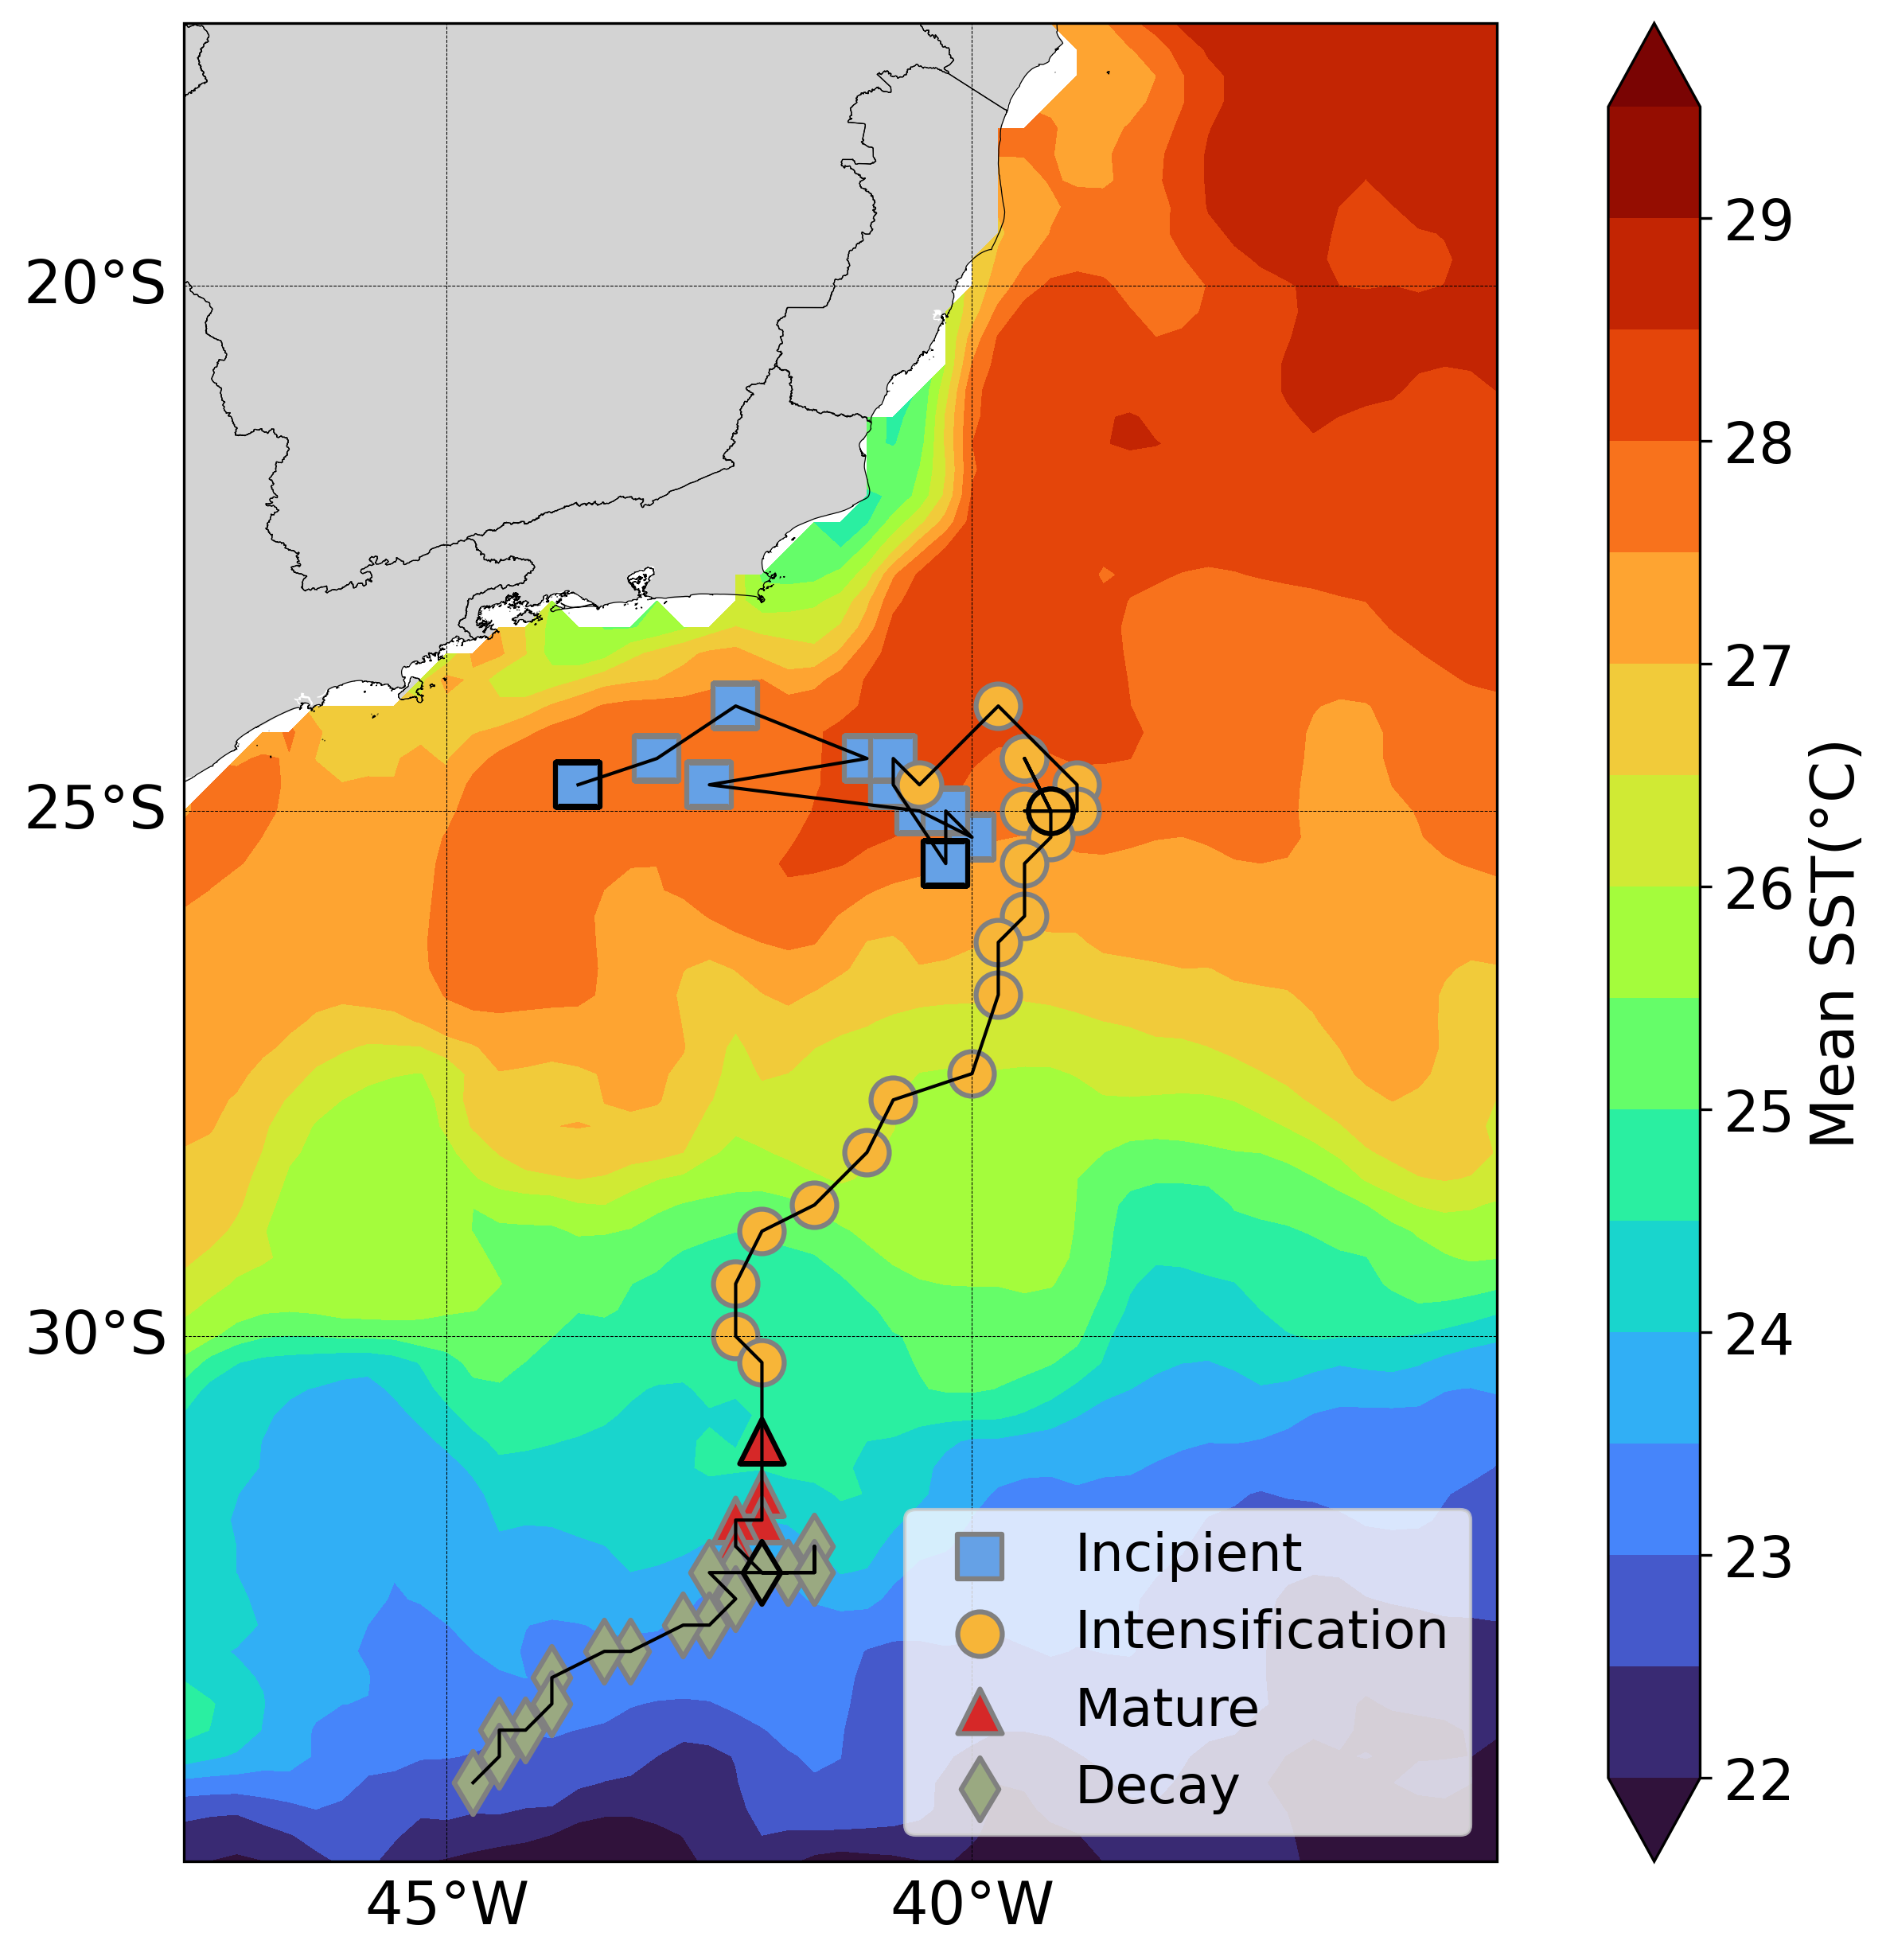
\includegraphics[width=\textwidth]{Akara_mean_sst_track.png}
\caption{Cyclone track and sea surface temperature (SST), expressed in $^{\circ}C$, averaged over the cyclone's duration from February 14 at 21Z to February 22 at 21Z. The track marker are color-coded to represent distinct phases of the cyclone's lifecycle. Enlarged markers indicate the dates corresponding to the snapshots shown in Figures \ref{fig:ch13}, \ref{fig:Akara_wind_speed_z500_composition}, and \ref{fig:Akara_mslp_sst_t2m_multiplot}.}
\label{fig:Akara_mean_sst_track}
\end{figure}

\subsection{Incipient Stage}

An advantage of utilizing relative vorticity, in addition to sea level pressure, for cyclone tracking is the ability to identify cyclogenesis before a closed isobar appears on surface charts \citep[e.g.,][]{sinclair1994objective,gramcianinov2019properties}. As demonstrated in \citet{couto2024new}, neglecting this early detection of the cyclone's incipient stage would result in the South Atlantic tracks being displaced eastward, farther from the continent. For instance, while \citet{reboita2024assessment} identified cyclogenesis at 12Z on February 15, in this study, it is detected earlier, at 21Z on February 14, during a period termed "Pre-cyclogenesis" by the authors.

\begin{figure}[h!]
    \centering
    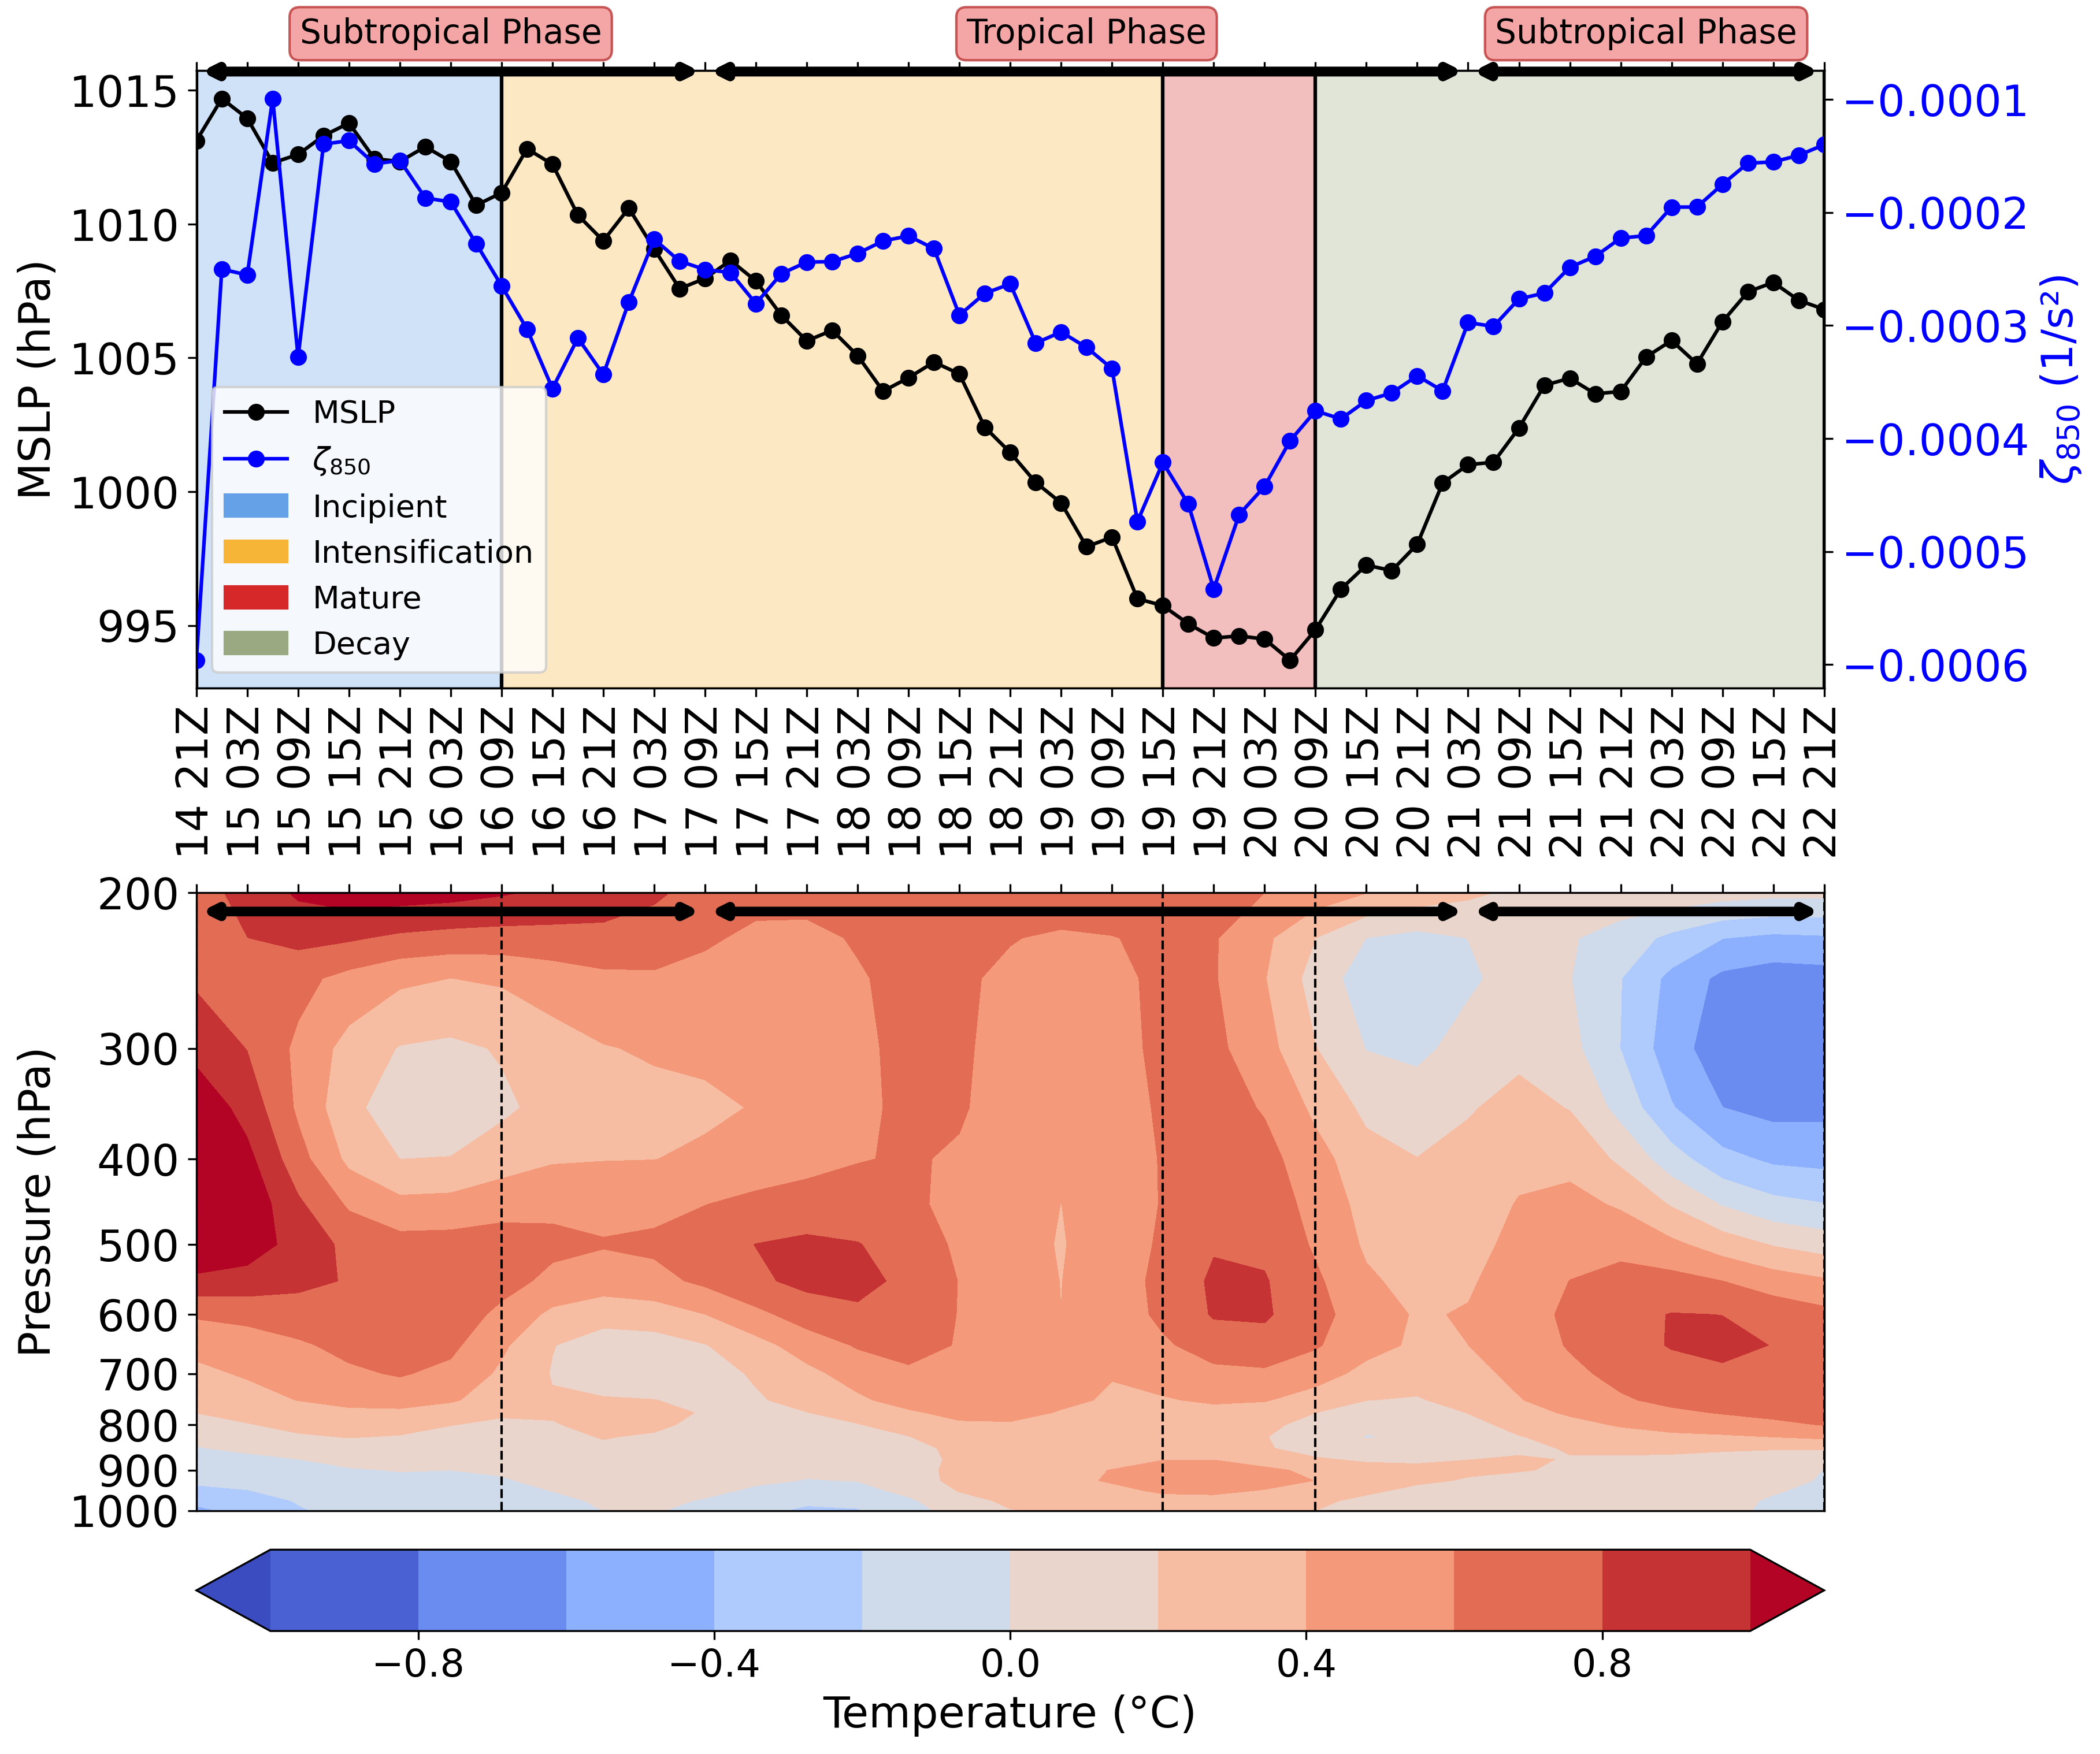
\includegraphics[width=\textwidth]{combined_serie_zonaldeviation.png}
    \caption{(Top) Time series of mean sea level pressure (MSLP, black line) and relative vorticity at 850 hPa ($\zeta_{850}$, blue line) at the cyclone center, as identified by the Cyclophaser program. Shaded areas represent the different phases of the cyclone's life cycle (incipient, intensification, mature, and decay), while the horizontal arrows indicate the subtropical and tropical phases. (Bottom) Vertical cross-section of the zonal mean temperature deviation ($\circ C$) near the cyclone center throughout the cyclone's life cycle. Dashed vertical lines indicate phase transitions: incipient to intensification, intensification to mature, and mature to decay. The horizontal arrows similarly indicate the subtropical and tropical phases.}
    \label{fig:combined_serie_zonaldeviation}
\end{figure}

As highlighted by \citet{reboita2024assessment}, cyclogenesis coincided with the passage of a cold front near Southeastern Brazil. On the beginning of the incipient stage, although the CPS indicates an symmetric deep cold core (Figure \ref{fig:cps}), the zonal temperature anomaly reveals an initially warm mid-upper troposphere (Figure \ref{fig:combined_serie_zonaldeviation}), attributed to deep convection in the frontal region (Figure \ref{fig:ch13}a). On February 15, a cutoff low begins to approach the surface cyclone (Figure \ref{fig:Akara_wind_speed_z500_composition}b), which subsequently moves southeastward. This interaction explains the relatively cold core observed in the mid-upper troposphere in Figure \ref{fig:combined_serie_zonaldeviation}. Additionally, the presence of a cutoff low at mid-upper levels is recognized as one of the primary mechanisms driving subtropical cyclogenesis \citep{da2019subtropical}. During this phase, the cyclone's thermal structure begins to evolve, as indicated by the CPS, transitioning toward a warmer and more symmetric system.

During the incipient phase (Figure \ref{fig:combined_serie_zonaldeviation}), the cyclone was located over relatively warm waters, with sea surface temperatures exceeding $28^{\circ}\text{C}$ (Figure \ref{fig:Akara_mean_sst_track}). Simultaneously, a thermal contrast of up to $3^{\circ}\text{C}$ between the ocean and the atmosphere near the cyclone center (Figure \ref{fig:Akara_mslp_sst_t2m_multiplot}a and \ref{fig:Akara_mslp_sst_t2m_multiplot}b) enhanced latent and sensible heat fluxes to the lower atmosphere. These fluxes reduced boundary layer stability \citep[e.g.,][]{pezzi2009multiyear,pezzi2021oceanic}, thereby promoting convective activity, as further evidenced by the vertical profile of horizontal vorticity advection (Figure \ref{fig:Vorticity_Budget_Combined_2x2}a): according to the quasi-geostrophic omega equation, increasing cyclonic (anticyclonic) vorticity advection with height induces upward (downward) motion \citep{trenberth1978interpretation,maddox1982examination}. 

Additionally, the positive $G_E$ term (Figure \ref{fig:lec}) and the diabatic heating term (Figure \ref{fig:Heat_Budget_Combined_2x2}a) indicate significant latent heat release associated with enhanced convective activity. While \citet{reboita2024assessment} suggested that warm advection by the South Atlantic Subtropical High (SASH) supported the cyclone's initial development, our analysis indicates that this contribution was negligible compared to other thermodynamic processes. Instead, diabatic heating was the primary contributors for heating the troposphere and, consequently, deepening the surface pressure. Meanwhile, adiabatic expansion due to the convective activity acted in the opposite direction, contributing for cooling the troposphere.  

The vorticity budget indicates a cyclonic tendency across all vertical levels during the incipient phase (Figure \ref{fig:Vorticity_Budget_Combined_2x2}a). Near the surface, the primary contributor to cyclonic vorticity is the relative vorticity component of the stretching term (ZD), which is associated with mass convergence. Between 900 hPa and 350 hPa, vertical advection emerges as the main contributor to the negative tendency, while above this layer, horizontal advection dominates. Throughout much of the lower and middle troposphere, vertical advection is largely canceled by the tilting term, a behavior similar to that observed for the South Atlantic subtropical cyclone Anita \citep{dutra2017structure}. Above 200 hPa, the planetary vorticity contribution to the stretching term (FD) surpasses ZD in magnitude, reflecting mass divergence. Although small in magnitude, the negative values of planetary vorticity advection throughout most of the atmospheric column indicate that the predominant meridional flow during this phase was northward, influenced by the post-frontal anticyclone. The small magnitude of the tilting term is associated with the weak wind shear in the Akará's environment, as demonstrated by \citet{reboita2024assessment}.

The LEC analysis for the incipient stage reveals that the barotropic conversion term $C_K$ ($K_Z \rightarrow K_E$) was the primary energy source driving cyclone (eddy) development (Figure \ref{fig:lec}a). In contrast, the baroclinic chain ($A_Z \rightarrow A_E \rightarrow K_E$) exhibited modest contributions, with $G_E$ being the dominant term supporting $K_E$. The low $C_A$ values align with the limited contribution from horizontal temperature advection in the heat budget, indicating weak meridional heat transport. Meanwhile, the moderate $G_Z$ and $C_E$ values are associated with ascending motions (and consequent latent heat release) in the frontal region (lower latitudes) and subsidence in the post-frontal region (higher latitudes).

\begin{figure}[h!]
\centering
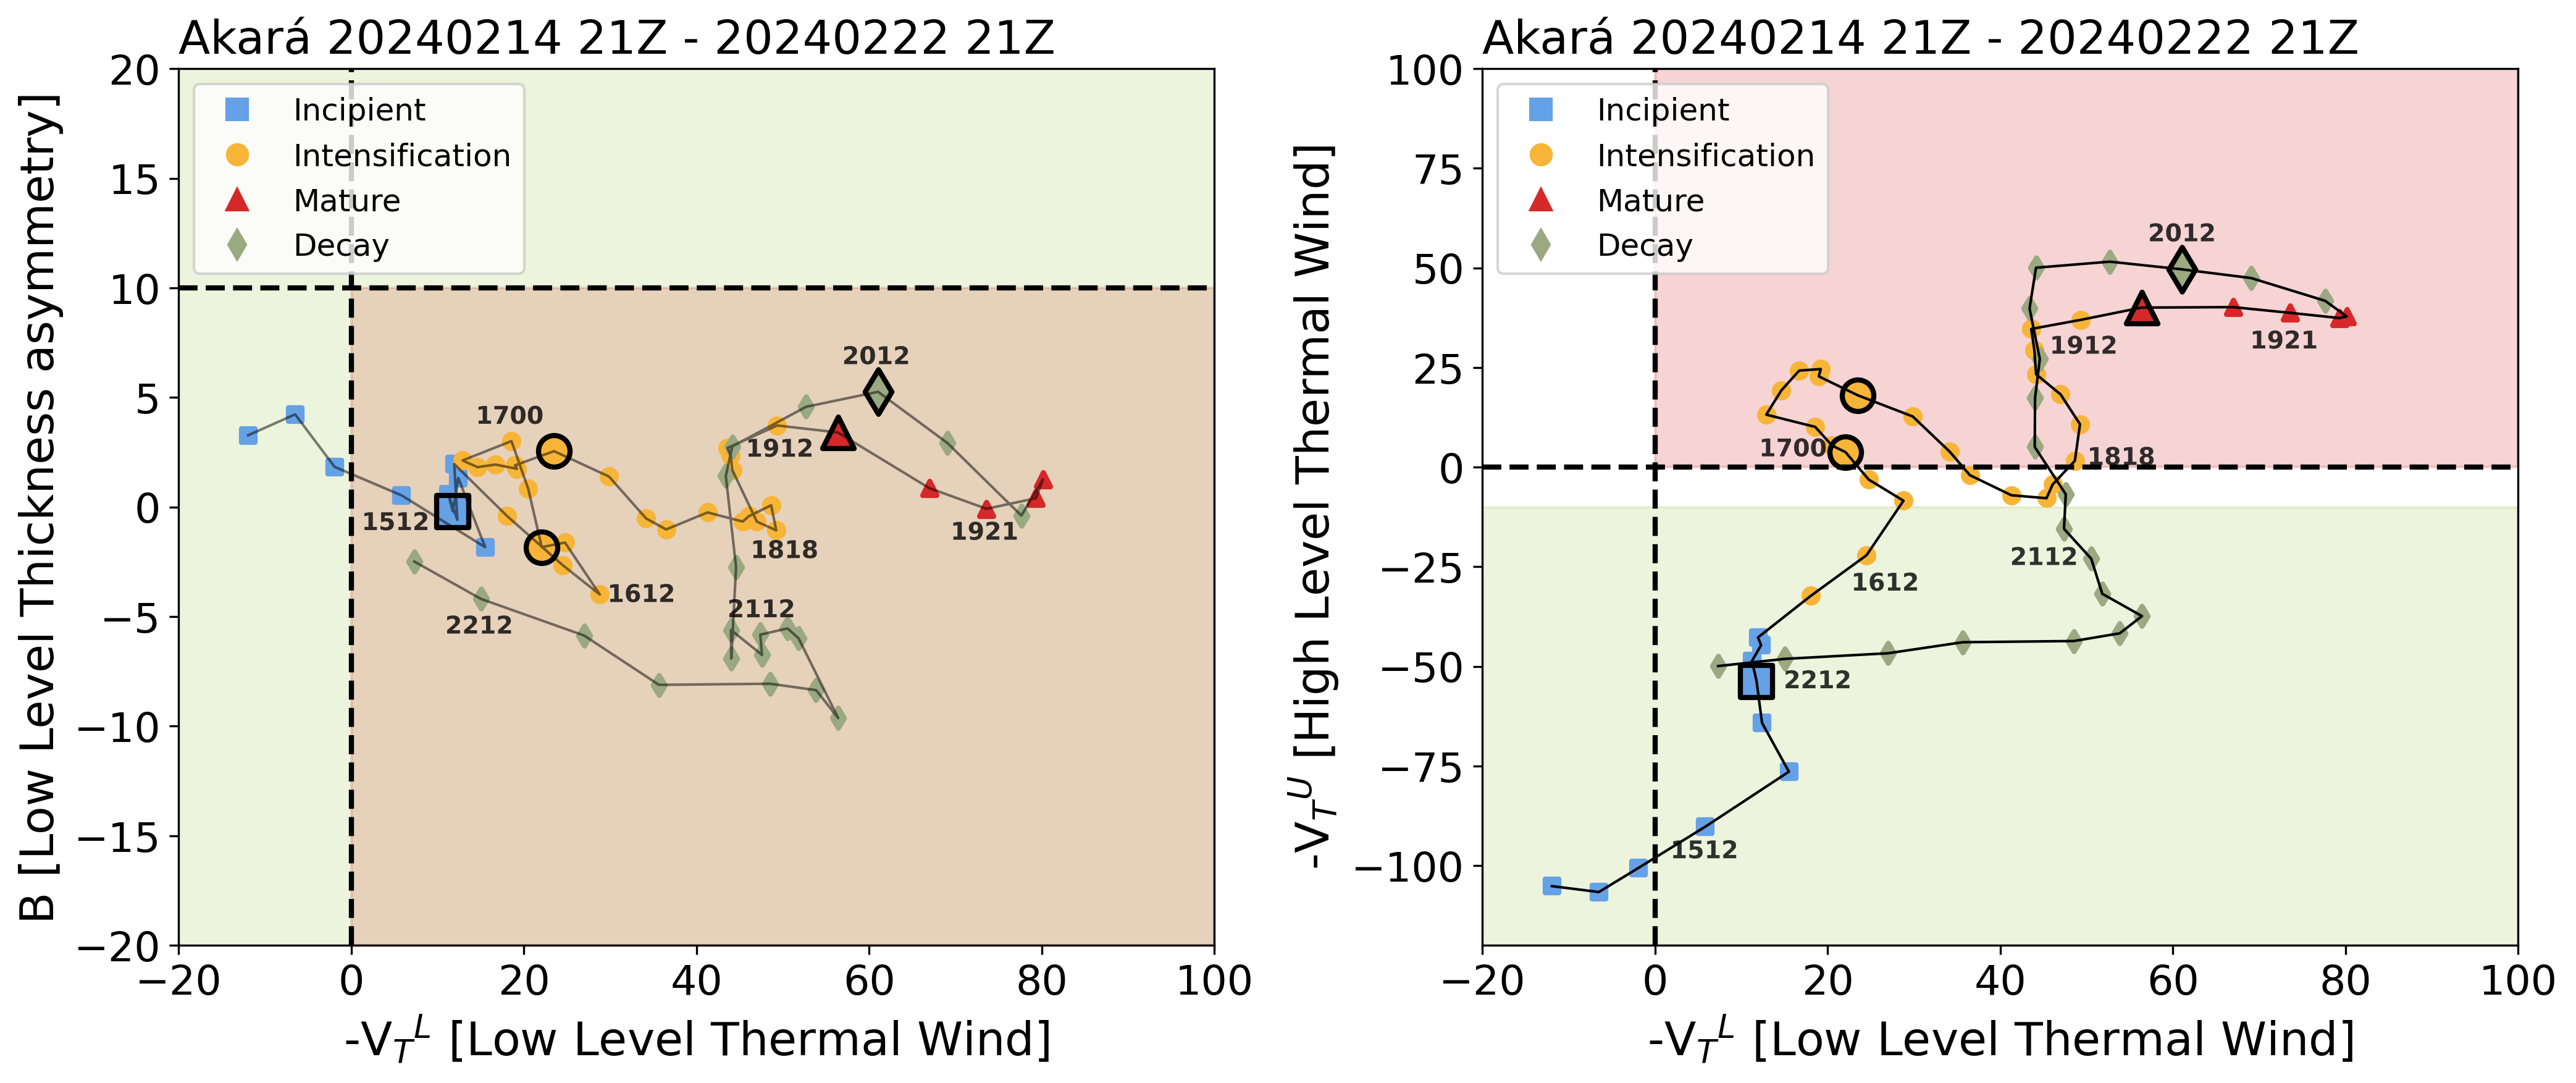
\includegraphics[width=\textwidth]{cps_datas_danilo.png}
\caption{Cyclone Phase Space (CPS) diagram for the Akará tropical transition from February 14 to February 22, 2024. (a) Low-level thickness asymmetry (\(B\)) and lower-tropospheric thermal wind (\(-V_T^L\)), (b) upper-tropospheric thermal wind (\(-V_T^U\)) and lower-tropospheric thermal wind (\(-V_T^L\)). Markers indicate distinct lifecycle phases, with annotations representing dates in day-hour format and enlarged markers indicate the dates corresponding to the snapshots shown in Figures \ref{fig:ch13}, \ref{fig:Akara_wind_speed_z500_composition}, and \ref{fig:Akara_mslp_sst_t2m_multiplot}. The background shading corresponds to phase classification thresholds for subtropical (based on Southern Atlantic criteria) and tropical cyclones.}
\label{fig:cps}
\end{figure}

Thus, during the incipient phase, the weak baroclinic environment near Akará provided energy to an upper-level jet structure, associated with a through (Figure \ref{fig:Akara_wind_speed_z500_composition}a), while also importing $K_Z$ from the boundaries. Most of the $K_Z$ was either converted into $K_E$ or dissipated through the residual term, leading to a sharp decrease in this component over time. These barotropic conversions were most intense in the mid-upper troposphere, especially between 300 and 400 hPa (Figure \ref{fig:SigmaOmega_Ck_combined_hov}). However, minor barotropic conversions occurred near the surface, related to the horizontal wind shear from the post-frontal and the SASH. Lastly, while some of the $K_E$ was lost through the residual term or exported out of the domain via $BK_E$, the fluxes from both $A_E$ and $K_Z$ contributed to a net increase in $K_E$ over time.

\begin{figure}[h!]
\centering
\includegraphics[width=\textwidth]{ch13.png}
\caption{Brightness temperature imagery from GOES-16 Channel 13 (shading), in $^{\circ}C$, and 1000 hPa wind barbels for distinct time steps of Akará's development, indicating the near-surface wind circulation associated with the cyclone.}
\label{fig:ch13}
\end{figure}

\begin{figure}[h!]
\centering
\includegraphics[width=\textwidth]{Akara_wind_speed_z500_composition.png}
\caption{Geopotential height at 500 hPa (red contours) and wind speed at 200 hPa (shaded, in m/s) at six distinct time steps during Akará's development. The black boxes represent the computational domain centered on the cyclone's position, used for the Lorenz Energy Cycle (LEC), heat budget, and vorticity budget analyses, while black crosses indicate the cyclone center.}
\label{fig:Akara_wind_speed_z500_composition}
\end{figure}

\subsection{Intensification Stage}

At the beginning of the intensification phase, at 09Z on February 16, the CPS already indicates a shallow, symmetric warm core (Figure \ref{fig:cps}), and the cyclone-related cloudiness begins to exhibit a spiral pattern (Figure \ref{fig:ch13}c). This shallow warm-core feature is also evident in the zonal mean temperature deviation field (Figure \ref{fig:combined_serie_zonaldeviation}), where a warm layer extends approximately between 800 and 400 hPa. Above this layer, a cold anomaly associated with the cutoff low persists until 15Z on February 17. During this period, the cyclone is located in a region with SSTs ranging from $27.5^{\circ}\text{C}$ to $28.5^{\circ}\text{C}$ (Figure \ref{fig:Akara_mean_sst_track}), but with a less intense air-sea temperature contrast (Figure \ref{fig:Akara_mslp_sst_t2m_multiplot}c). 

Despite this, there is an increase in mass convergence near the surface, as shown by the ZD term (Figure \ref{fig:Vorticity_Budget_Combined_2x2}b), further promoting convective activity. Similar to the incipient phase, the vorticity advection profile — anticyclonic near the surface and cyclonic near 200 hPa — is favorable for upward motion. The resulting convective activity leads to an increase in the magnitude of both the diabatic heating term (Figure \ref{fig:Heat_Budget_Combined_2x2}b) and the $G_E$ term (Figure \ref{fig:lec}b) compared to the incipient stage.

Consequently, there is a tendency for heating throughout most of the atmospheric column, especially in the mid-troposphere (Figure \ref{fig:Heat_Budget_Combined_2x2}b). Although the total vertical motion effect term partially counterbalances the diabatic term during the intensification phase, the diabatic term dominates, contributing to the observed heating. This heating on the cutoff low layer is primarily attributed to latent heat release from convective activity. Meanwhile, horizontal temperature advection is negligible up to approximately 200 hPa. Above this level, while the magnitude of this term increases, adiabatic cooling and the vanishing diabatic term result in net cooling in the upper troposphere, as observed in Figure \ref{fig:combined_serie_zonaldeviation}. Lastly, from a quasi-geostrophic perspective, the vertical derivative of the diabatic term contributes to lowering geopotential height in a deep layer near the surface.


\begin{figure}[h!]
\centering
\includegraphics[width=\textwidth]{Akara_mslp_sst_t2m_multiplot.png}
\caption{Difference between sea surface temperature and 2-meter air temperature (SST - T2M, shaded) and mean sea level pressure (SLP, white contours in hPa) at six distinct time steps during Akará's development. The black crosses indicate the cyclone center at each time step.}
\label{fig:Akara_mslp_sst_t2m_multiplot}
\end{figure}

\begin{figure}[h!]
\centering
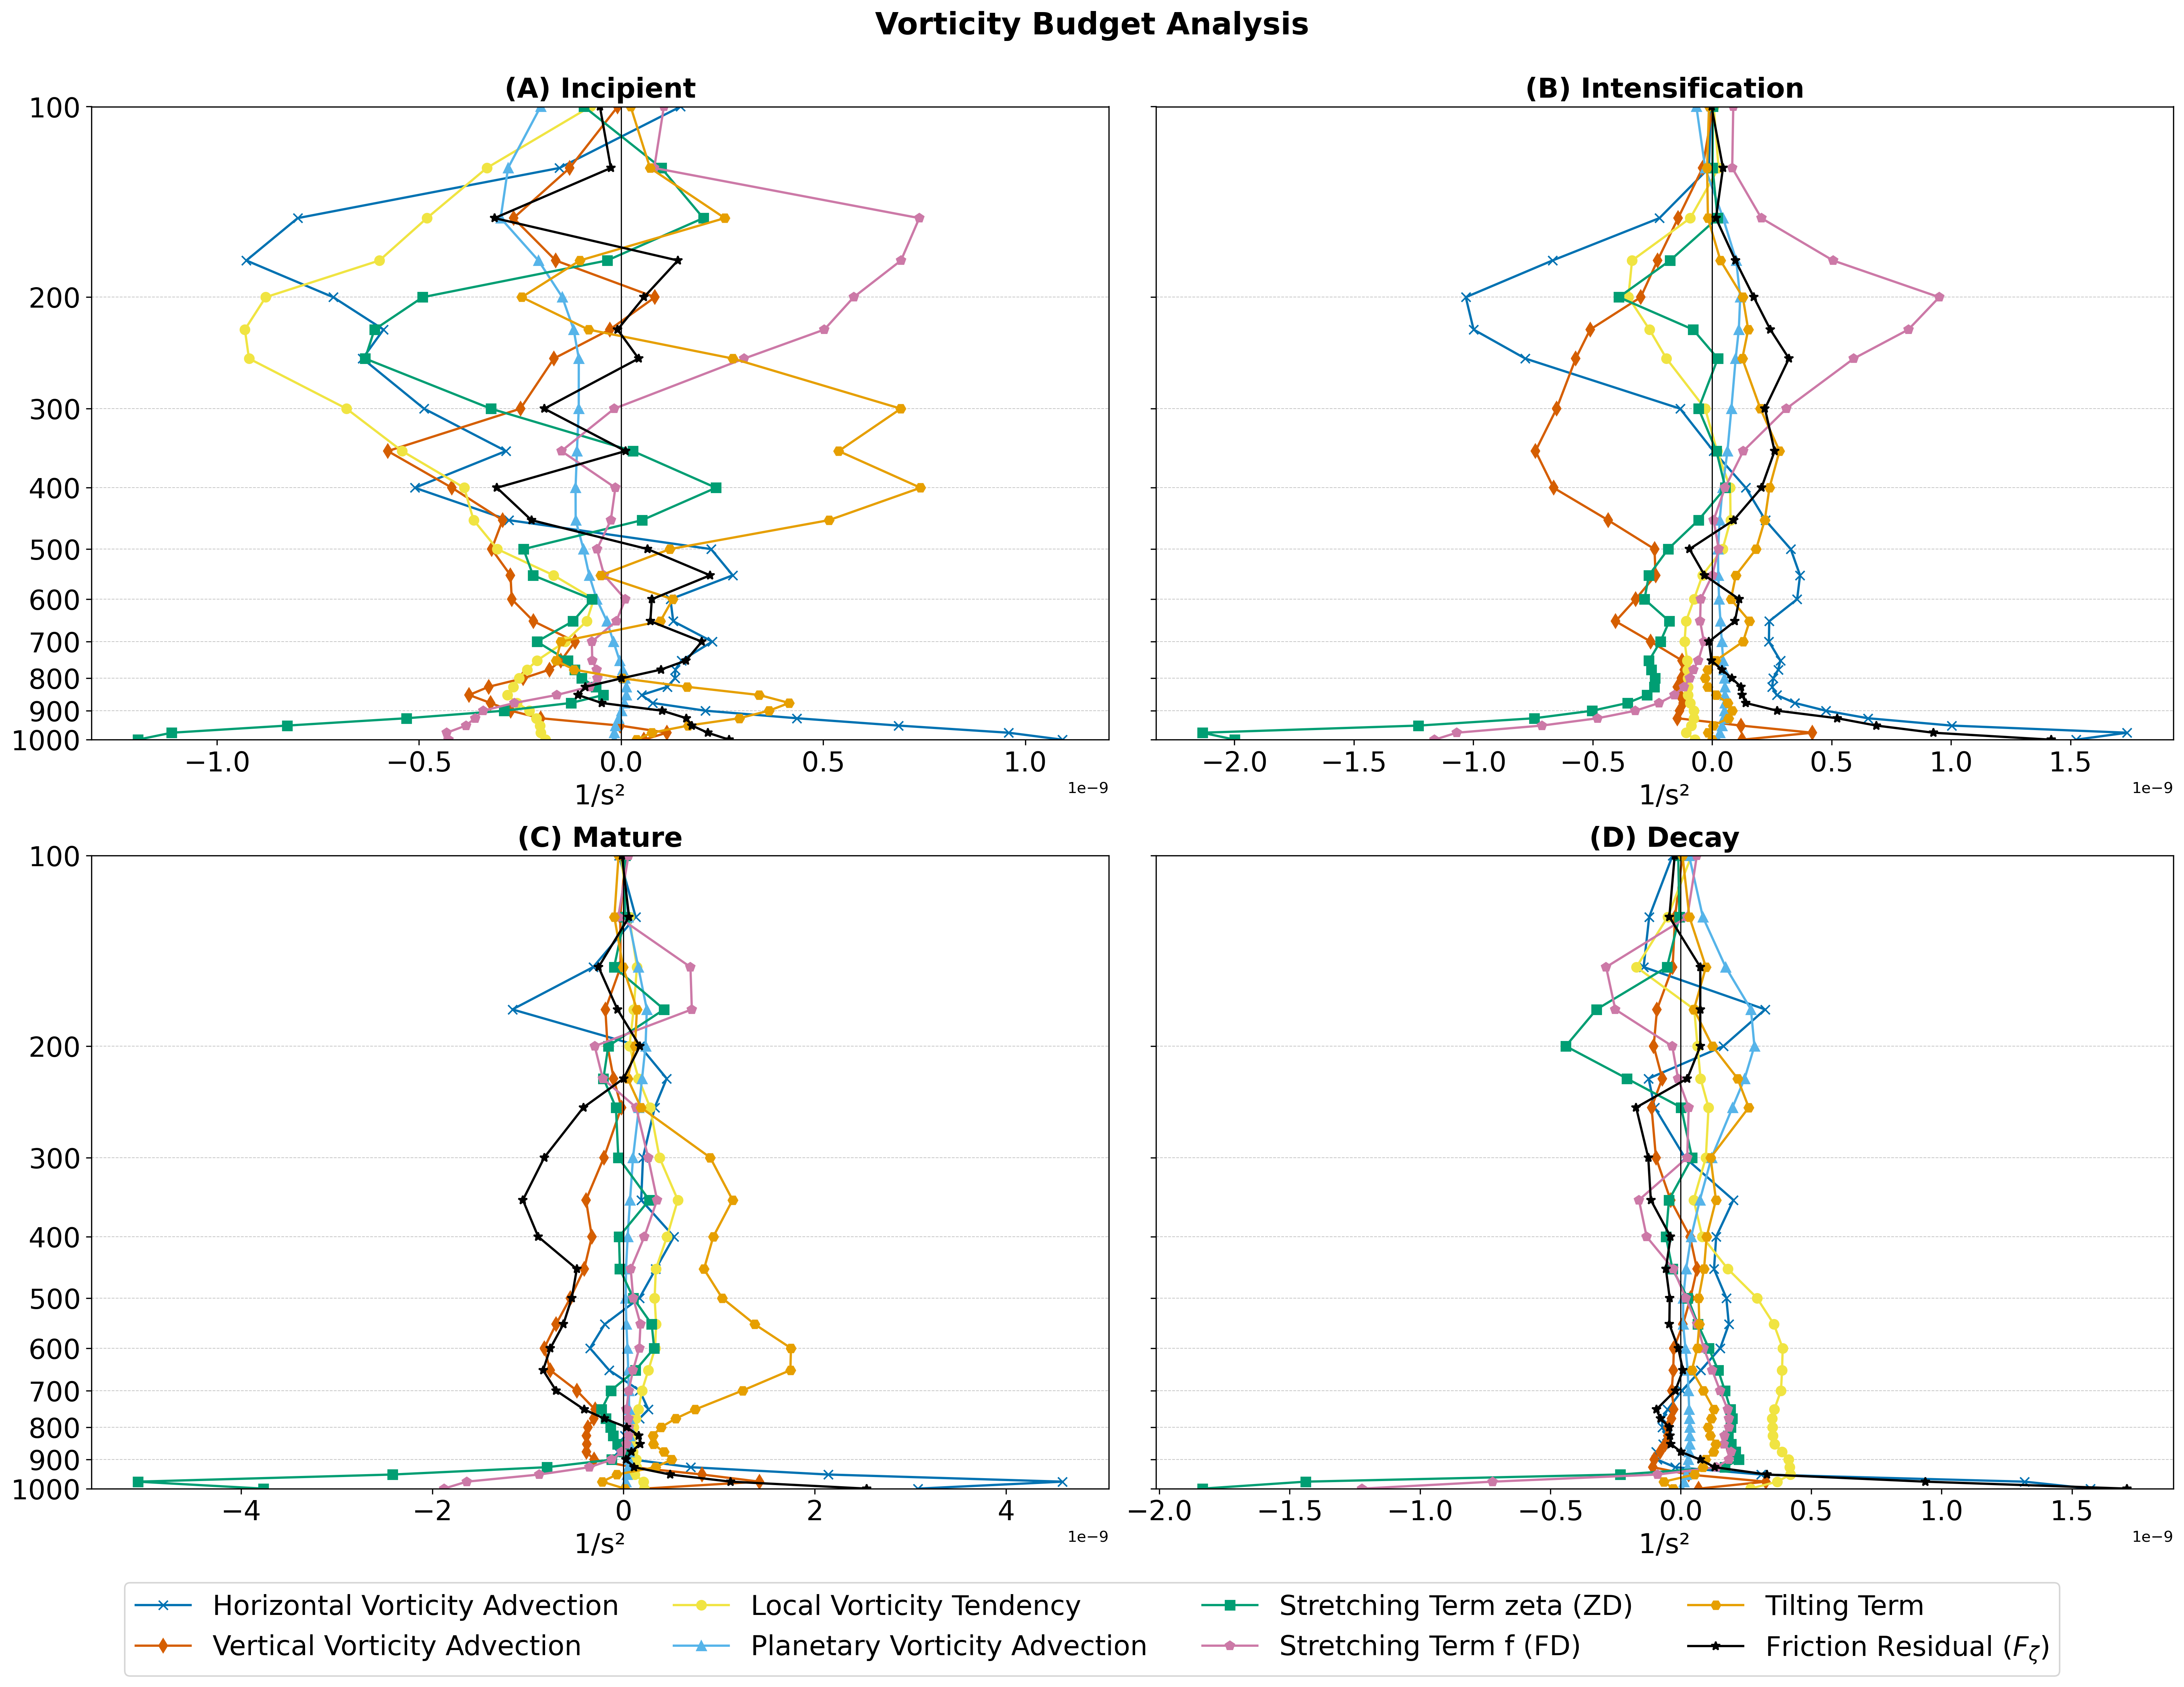
\includegraphics[width=\textwidth]{Vorticity_Budget_Combined_2x2.png}
\caption{Vertical profiles of the vorticity budget terms during the distinct phases of the Akará lifecycle: (a) Incipient, (b) Intensification, (c) Mature, and (d) Decay, expressed in s\(^{-2}\).}
\label{fig:Vorticity_Budget_Combined_2x2}
\end{figure}

Regarding the vorticity budget, the cyclonic vorticity tendency at both lower and upper levels is smaller than during the incipient phase (Figure \ref{fig:Vorticity_Budget_Combined_2x2}b). Near the surface, the FD and especially the ZD terms are intense contributors to cyclonic vorticity, indicating mass convergence, although they are largely offset by anticyclonic advection and the friction term. The vertical vorticity advection increases in magnitude compared to the incipient stage, particularly between 500 and 200 hPa, where it becomes the primary contributor to cyclonic circulation from 900 hPa to approximately 250 hPa. Above this level, cyclonic horizontal vorticity advection dominates and ZD indicates mass divergence, fostering the vertical ascent. Although planetary vorticity advection becomes positive during this phase, indicating predominantly southward flow as the anticyclonic flow weakens, its magnitude remains negligible compared to other terms.

The observed cyclonic tendency at mid-upper levels intensifies the mid-upper-level cyclonic structure (Figure \ref{fig:Akara_wind_speed_z500_composition}c). Additionally, the tilting term is weaker than during the incipient stage as the cyclone moves southward toward the frontal region, coinciding with a decrease in vertical wind shear \citep{reboita2024assessment}. At this stage, Akará already exhibits a barotropic structure.

In addition to the cyclone's barotropic structure, its environment also becomes more barotropic during the intensification phase. This is reflected in the LEC, which shows a sharp decrease in the $C_Z$ term and the baroclinic conversion term $C_A$. Consequently, the primary energy source for $C_E$ is the $G_E$ term, associated with latent heat release. At the same time, barotropic conversions increase, with $C_K$ becoming more negative. Notably, barotropic conversions are the primary energy sources driving Akará's intensification. During this phase, there is also a sharp increase in the $K_E$ budget, indicating system intensification, accompanied by a twofold increase in the $RK_E$ term, linked to increased frictional dissipation, as indicated by the $F_{\zeta}$ term (Figure \ref{fig:Vorticity_Budget_Combined_2x2}b). The increase in the friction near the surface also helps on promoting mass convergence and therefore upward motion, due to the effect of Ekman pumping on the boundary layer \citep[e.g.,]{hamouda2019ekman}.

By February 17, the entire tropospheric column becomes warm (Figure \ref{fig:combined_serie_zonaldeviation}), marking the system's tropical transition \citep{wood2023phase,reboita2024assessment}. This transition is further confirmed by the CPS, where the \(V_T^L\) and \(V_T^U\) parameters indicate the development of a deep warm core (Figure \ref{fig:cps}b). Although diabatic heating significantly contributes to this warming, as discussed earlier in this section and by \citet{reboita2024assessment}, an important contribution is neglected when only low-level forcing is considered, as discussed below.

After the tropical transition, while Akará is still over warm waters, above 27 $^{\circ}C$ (Figure \ref{fig:Akara_mean_sst_track}), it transitions to relatively cool atmospheric region than during the subtropical phase, with a higher thermal contrast between the ocean and the atmosphere (Figure \ref{fig:Akara_mslp_sst_t2m_multiplot}d). Meanwhile, examination of the total vertical motion effect term (Figure \ref{fig:SigmaOmega_Ck_combined_hov}) indicates evidence of stratospheric air intrusion. This is marked by subsidence beginning on February 17 near 10 hPa and reaching down to approximately 200 hPa. This process further intensifies the mid-upper-level low (Figure \ref{fig:Akara_wind_speed_z500_composition}d), increasing mass divergence at upper levels, as indicated by the FD profile (\textbf{supplementary figure: hovmoller-fDivH}). Ultimately, these features promote convective activity, increasing latent heat release and contributing to the warming of the tropospheric column. Furthermore, as the jet-like feature moves away from the region, the peak $C_K$ conversions shift from the upper troposphere to the surface (Figure \ref{fig:SigmaOmega_Ck_combined_hov}). This is possibly associated with increased horizontal wind shear resulting from the convergence of the southwesterly flow from the post-frontal high and the northeasterly flow from the SASH near the cyclone center (Figure \ref{fig:ch13}d).

\begin{figure}[h!]
\centering
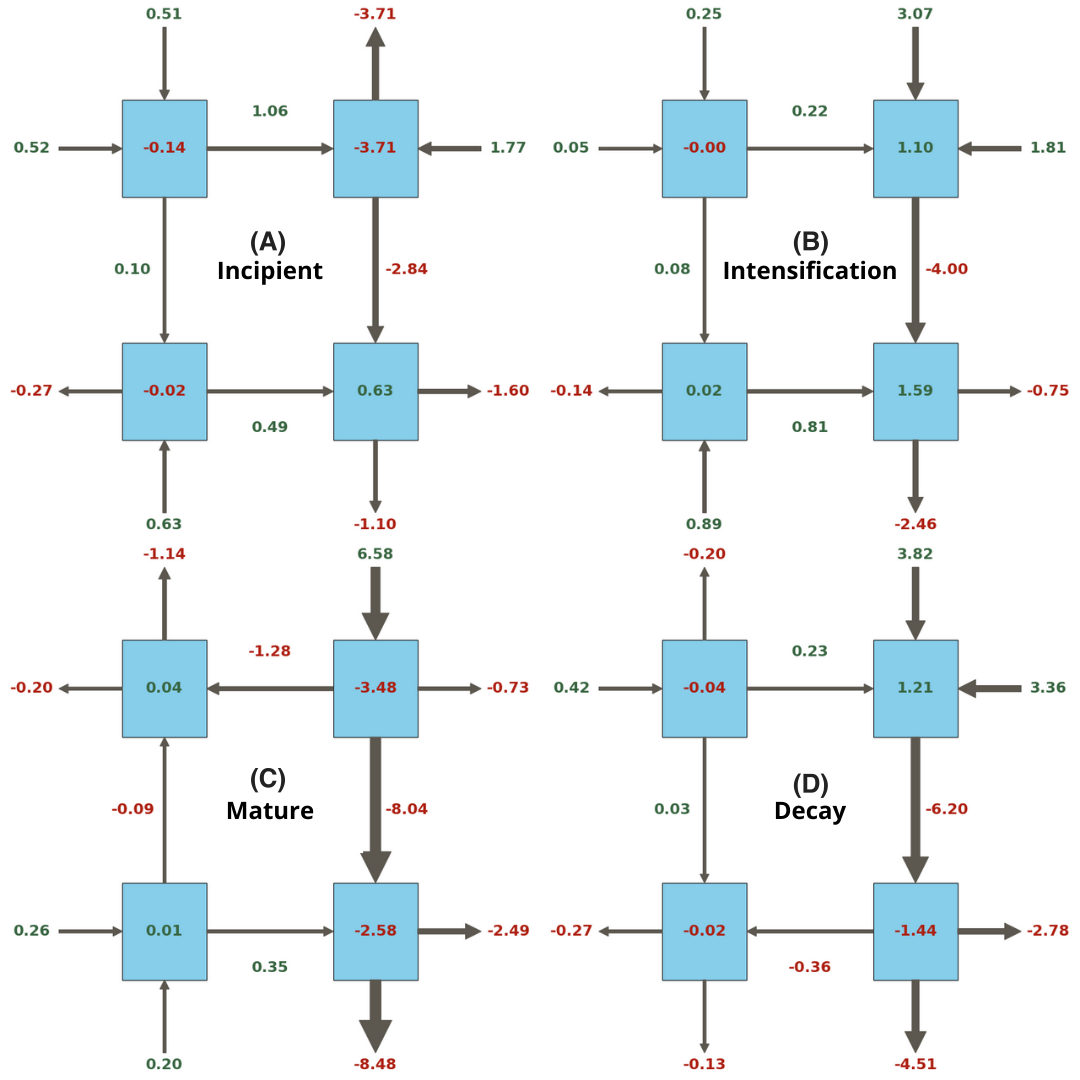
\includegraphics[width=\textwidth]{lec.png}
\caption{Lorenz Energy Cycle (LEC) diagrams representing the energy exchanges during each phase of the Akará lifecycle: (a) Incipient, (b) Intensification, (c) Mature, and (d) Decay. The blue boxes represent the energy reservoirs for zonal and eddy components of available potential energy (APE) and kinetic energy (KE). Arrows indicate the direction and magnitude of energy conversions between these reservoirs, with positive values in green and negative values in red, expressed in units of W m\(^{-2}\). The terms are defined in Figure \ref{fig:LEC_example}.}
\label{fig:lec}
\end{figure}


\subsection{Mature Stage}

During the mature phase, the CPS continues to indicate a deep warm-core structure (Figure \ref{fig:cps}b). This structure becomes even more pronounced compared to the intensification phase, as shown in Figure \ref{fig:combined_serie_zonaldeviation}. The surface layer becomes relatively warm, with a particularly notable warming between 600 and 500 hPa. Meanwhile, the cyclone's southward displacement brings it close to relatively cold waters (Figures \ref{fig:Akara_mean_sst_track} and \ref{fig:Akara_mslp_sst_t2m_multiplot}e), which stabilize the boundary layer, suppressing convection.

Despite a significant increase in anticyclonic vorticity advection near the surface compared to the previous phase, cyclonic advection is now confined to two layers: between 700 and 500 hPa and between 200 and 150 hPa (Figure \ref{fig:Vorticity_Budget_Combined_2x2}c). From a quasi-geostrophic perspective, this configuration indicates an environment less favorable for vertical motion than during the intensification phase. Consequently, the positive values of the diabatic term become confined below the 300 hPa layer and decrease in mean magnitude (Figure \ref{fig:Heat_Budget_Combined_2x2}c). Similarly, the $G_E$ term experiences a sharp decrease in magnitude. This reduction in convective activity is also visible in satellite imagery, which, despite displaying symmetric cloudiness around the cyclone center, shows lower cloud tops compared to previous phases (Figure \ref{fig:ch13}e).

The decrease in convective activity results in a cooling tendency above 400 hPa, despite a warming tendency below this level (Figure \ref{fig:Heat_Budget_Combined_2x2}c). The warming below 400 hPa is supported by an increase in horizontal temperature advection, particularly above 800 hPa, where the total vertical motion effect nearly offsets the diabatic term. Above 200 hPa, a sharp increase in warm advection leads to a net warming tendency in the upper troposphere. 

\begin{figure}[h!]
\centering
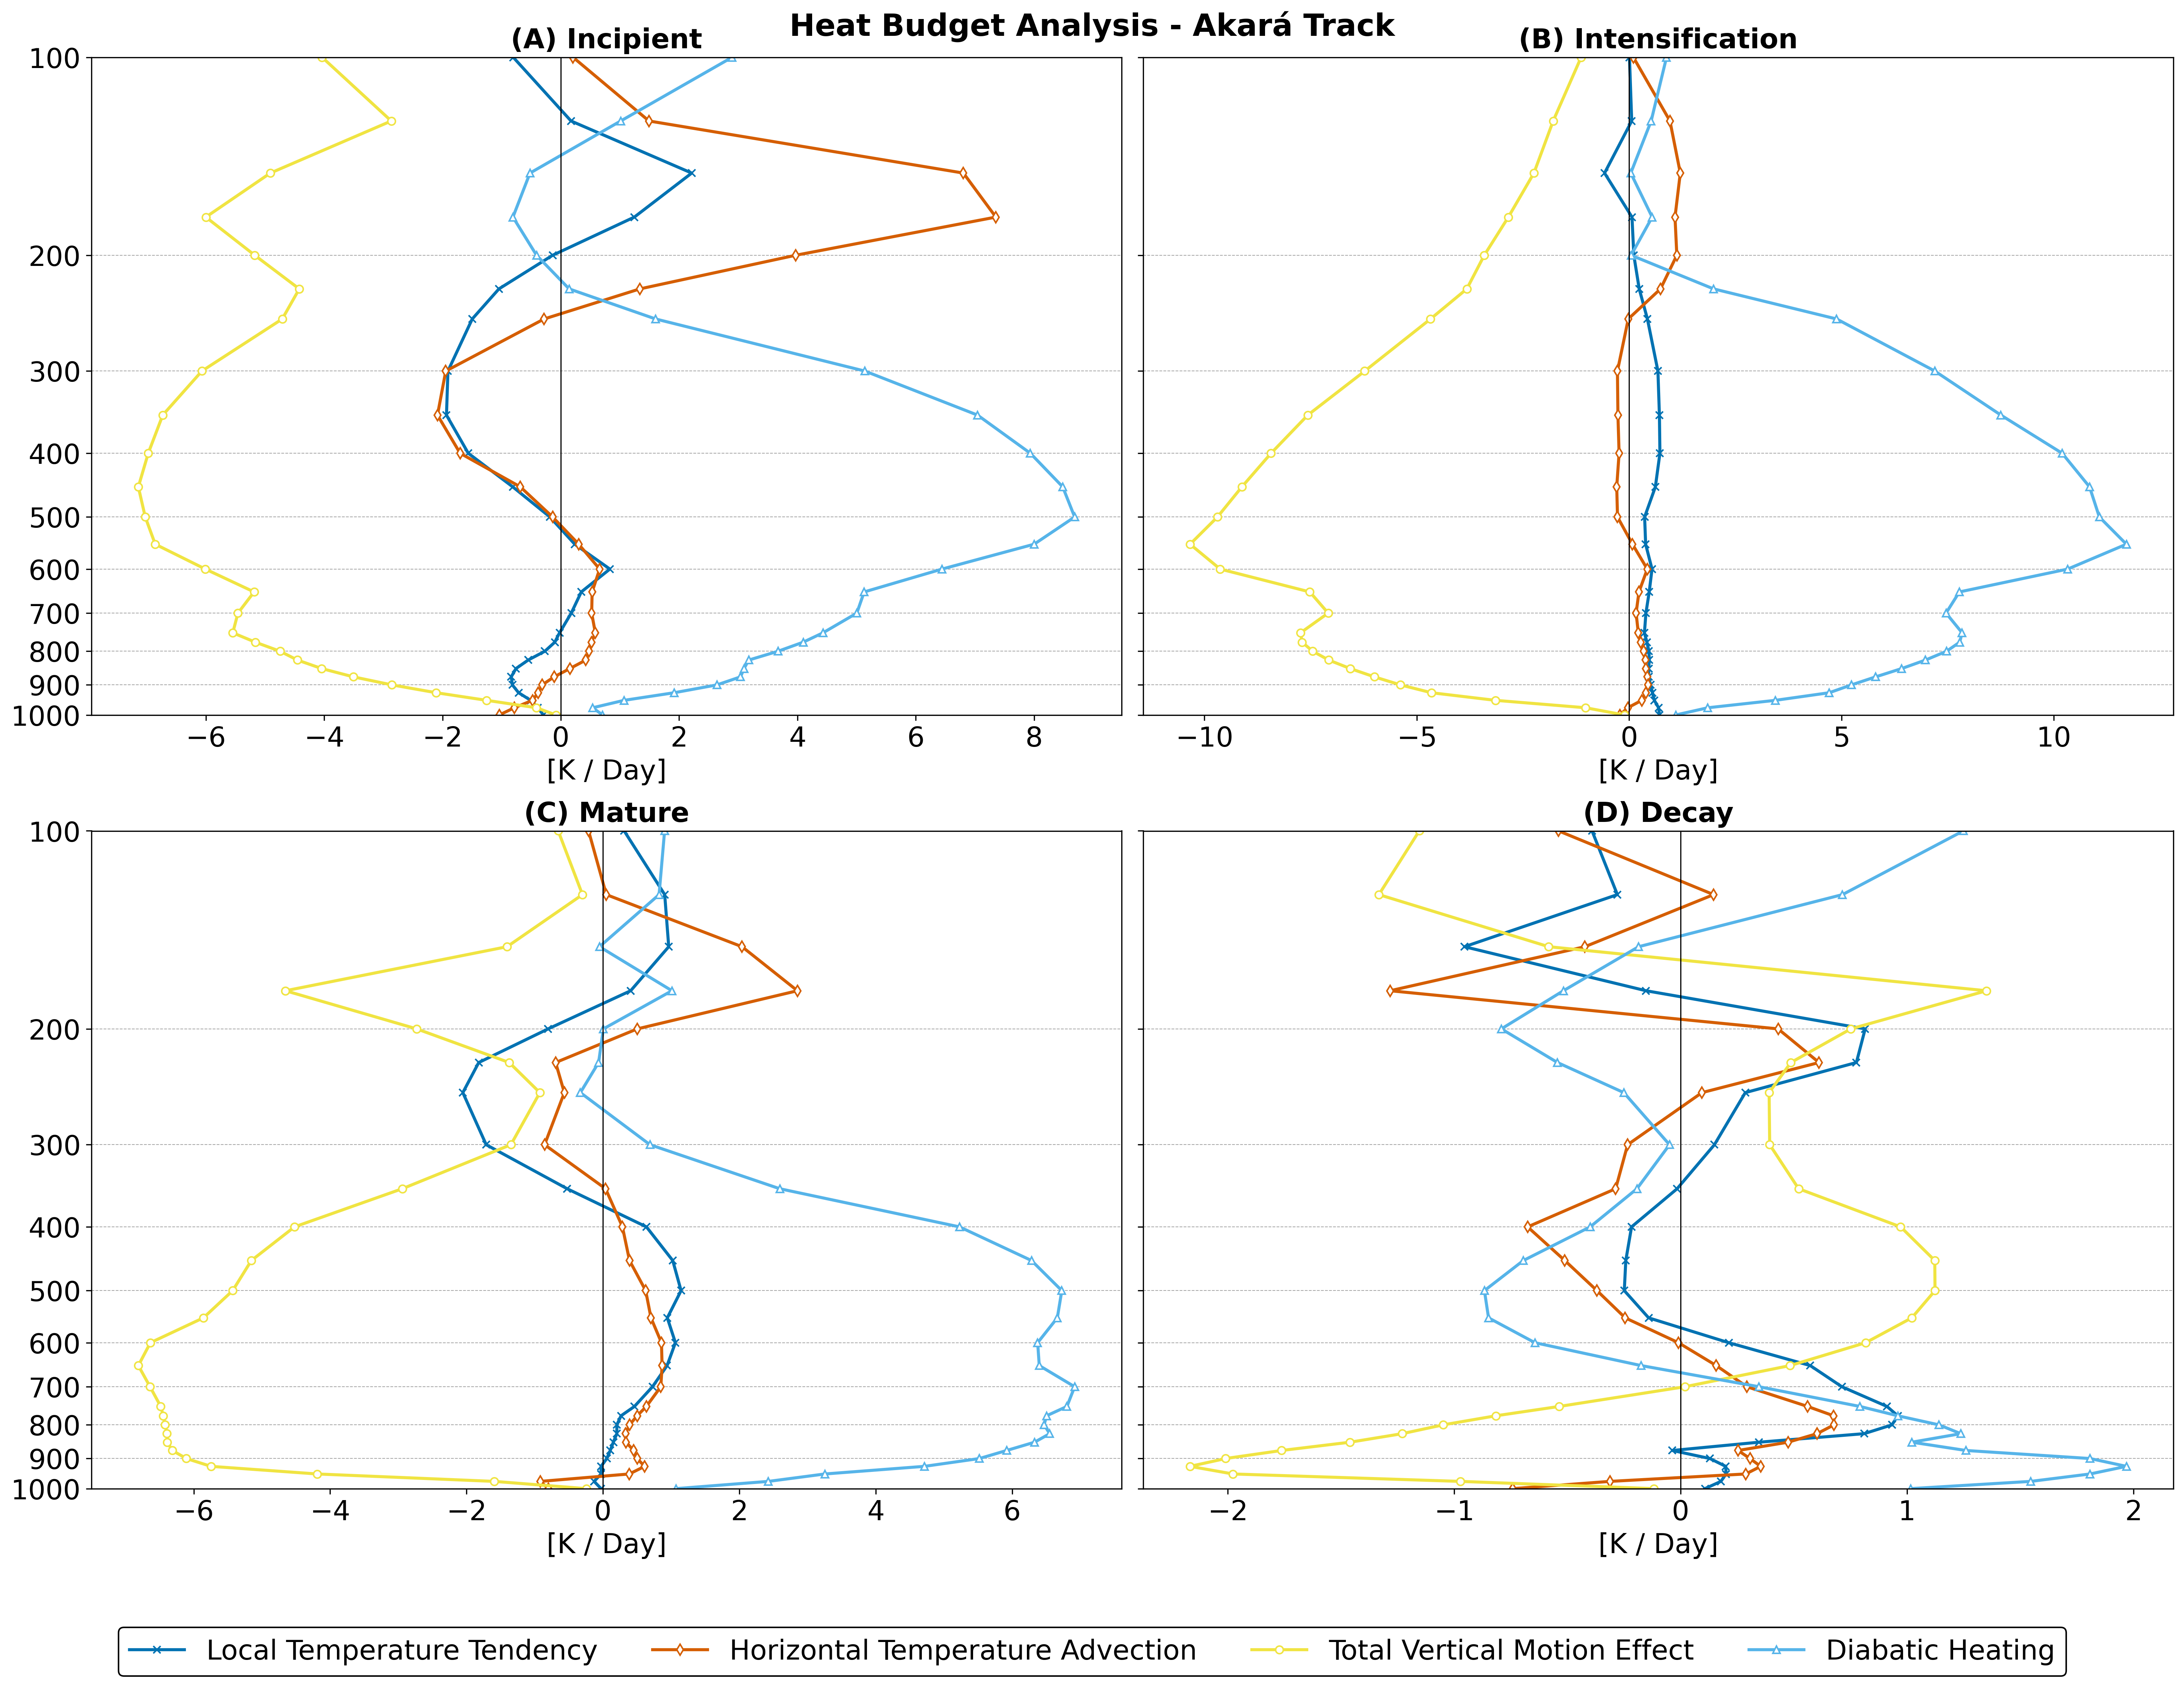
\includegraphics[width=\textwidth]{Heat_Budget_Combined_2x2.png}
\caption{Vertical profiles of the heat budget terms during the distinct phases of the Akará lifecycle: (a) Incipient, (b) Intensification, (c) Mature, and (d) Decay, expressed in K/day.}
\label{fig:Heat_Budget_Combined_2x2}
\end{figure}

Although the time-averaged total vertical motion effect term indicates a net cooling contribution, the influence of stratospheric intrusion becomes evident (Figure \ref{fig:SigmaOmega_Ck_combined_hov}). This interaction promotes a warming effect that propagates downward from the upper atmospheric layers to approximately 300 hPa. Consequently, the surface fluxes, although present, were insufficient to sustain deep convective activity capable of warming the upper troposphere. Instead, the stratosphere-troposphere interactions played a significant role in contributing to the observed warming of the mid-upper troposphere.

At this stage, a moderate anticyclonic tendency is observed throughout the troposphere, consistent with the system no longer intensifying. Near the surface, FD and especially ZD strongly contribute to cyclonic tendencies, indicating mass convergence, but these are counterbalanced by intense anticyclonic horizontal advection and the residual term. Throughout most of the atmospheric column up to 200 hPa, the residual term and vertical vorticity advection contribute cyclonically but are offset by the tilting term, which shows a sharp increase in magnitude compared to previous phases. As discussed by \citet{dutra2017structure}, the tilting term is often negligible in synoptic-scale motions, but its prominence in Akará's mature phase indicates the system's mesoscale characteristics as a tropical cyclone. Its high values also suggest increased vertical wind shear, driven by intense surface winds \citep{reboita2024assessment}. Above 200 hPa, FD becomes the primary contributor to the anticyclonic tendency, indicating mass divergence, albeit confined to a narrower layer compared to earlier phases.

From an energetic perspective, Akará's environment becomes fully barotropic, characterized by negative $C_Z$ and $C_A$ conversions. These terms reflect a reduction in environmental north-south temperature gradients, despite ongoing meridional heat transport and residual convective activity (Figure \ref{fig:ch13}e). Barotropic conversions, similar to the intensification phase, remain the primary energy source for Akará, with a twofold increase in magnitude. This is accompanied by a comparable increase in the $RK_Z$ term and a fourfold increase in $RK_E$. The increase in $RK_E$ is associated with higher dissipation rates, as indicated by the $F_{\zeta}$ term, which transfers momentum to the sea surface and generates high sea waves \citep[e.g.,]{zhao2022effects,shimura2024footprint}. For $RK_Z$, the large values may be linked to energy upscale transfer from subgrid to grid-scale processes, as suggested by \citet{michaelides1987limited}. However, since this term also includes numerical errors and other unresolved processes, this interpretation remains speculative. 

The dissipation of $K_E$, combined with energy exports, results in an overall negative budget for this term as the system reaches its maximum intensity and transitions into the decay stage. Notably, barotropic conversions during the mature phase occur throughout almost the entire troposphere, with strong values extending from near the surface up to 500 hPa (Figure \ref{fig:SigmaOmega_Ck_combined_hov}). These conversions may have been enhanced by the strong horizontal wind shear near the cyclone center as it reached peak intensity, as well as by vertical wind shear, as evidenced by the tilting term.

\begin{figure}[h!]
\centering
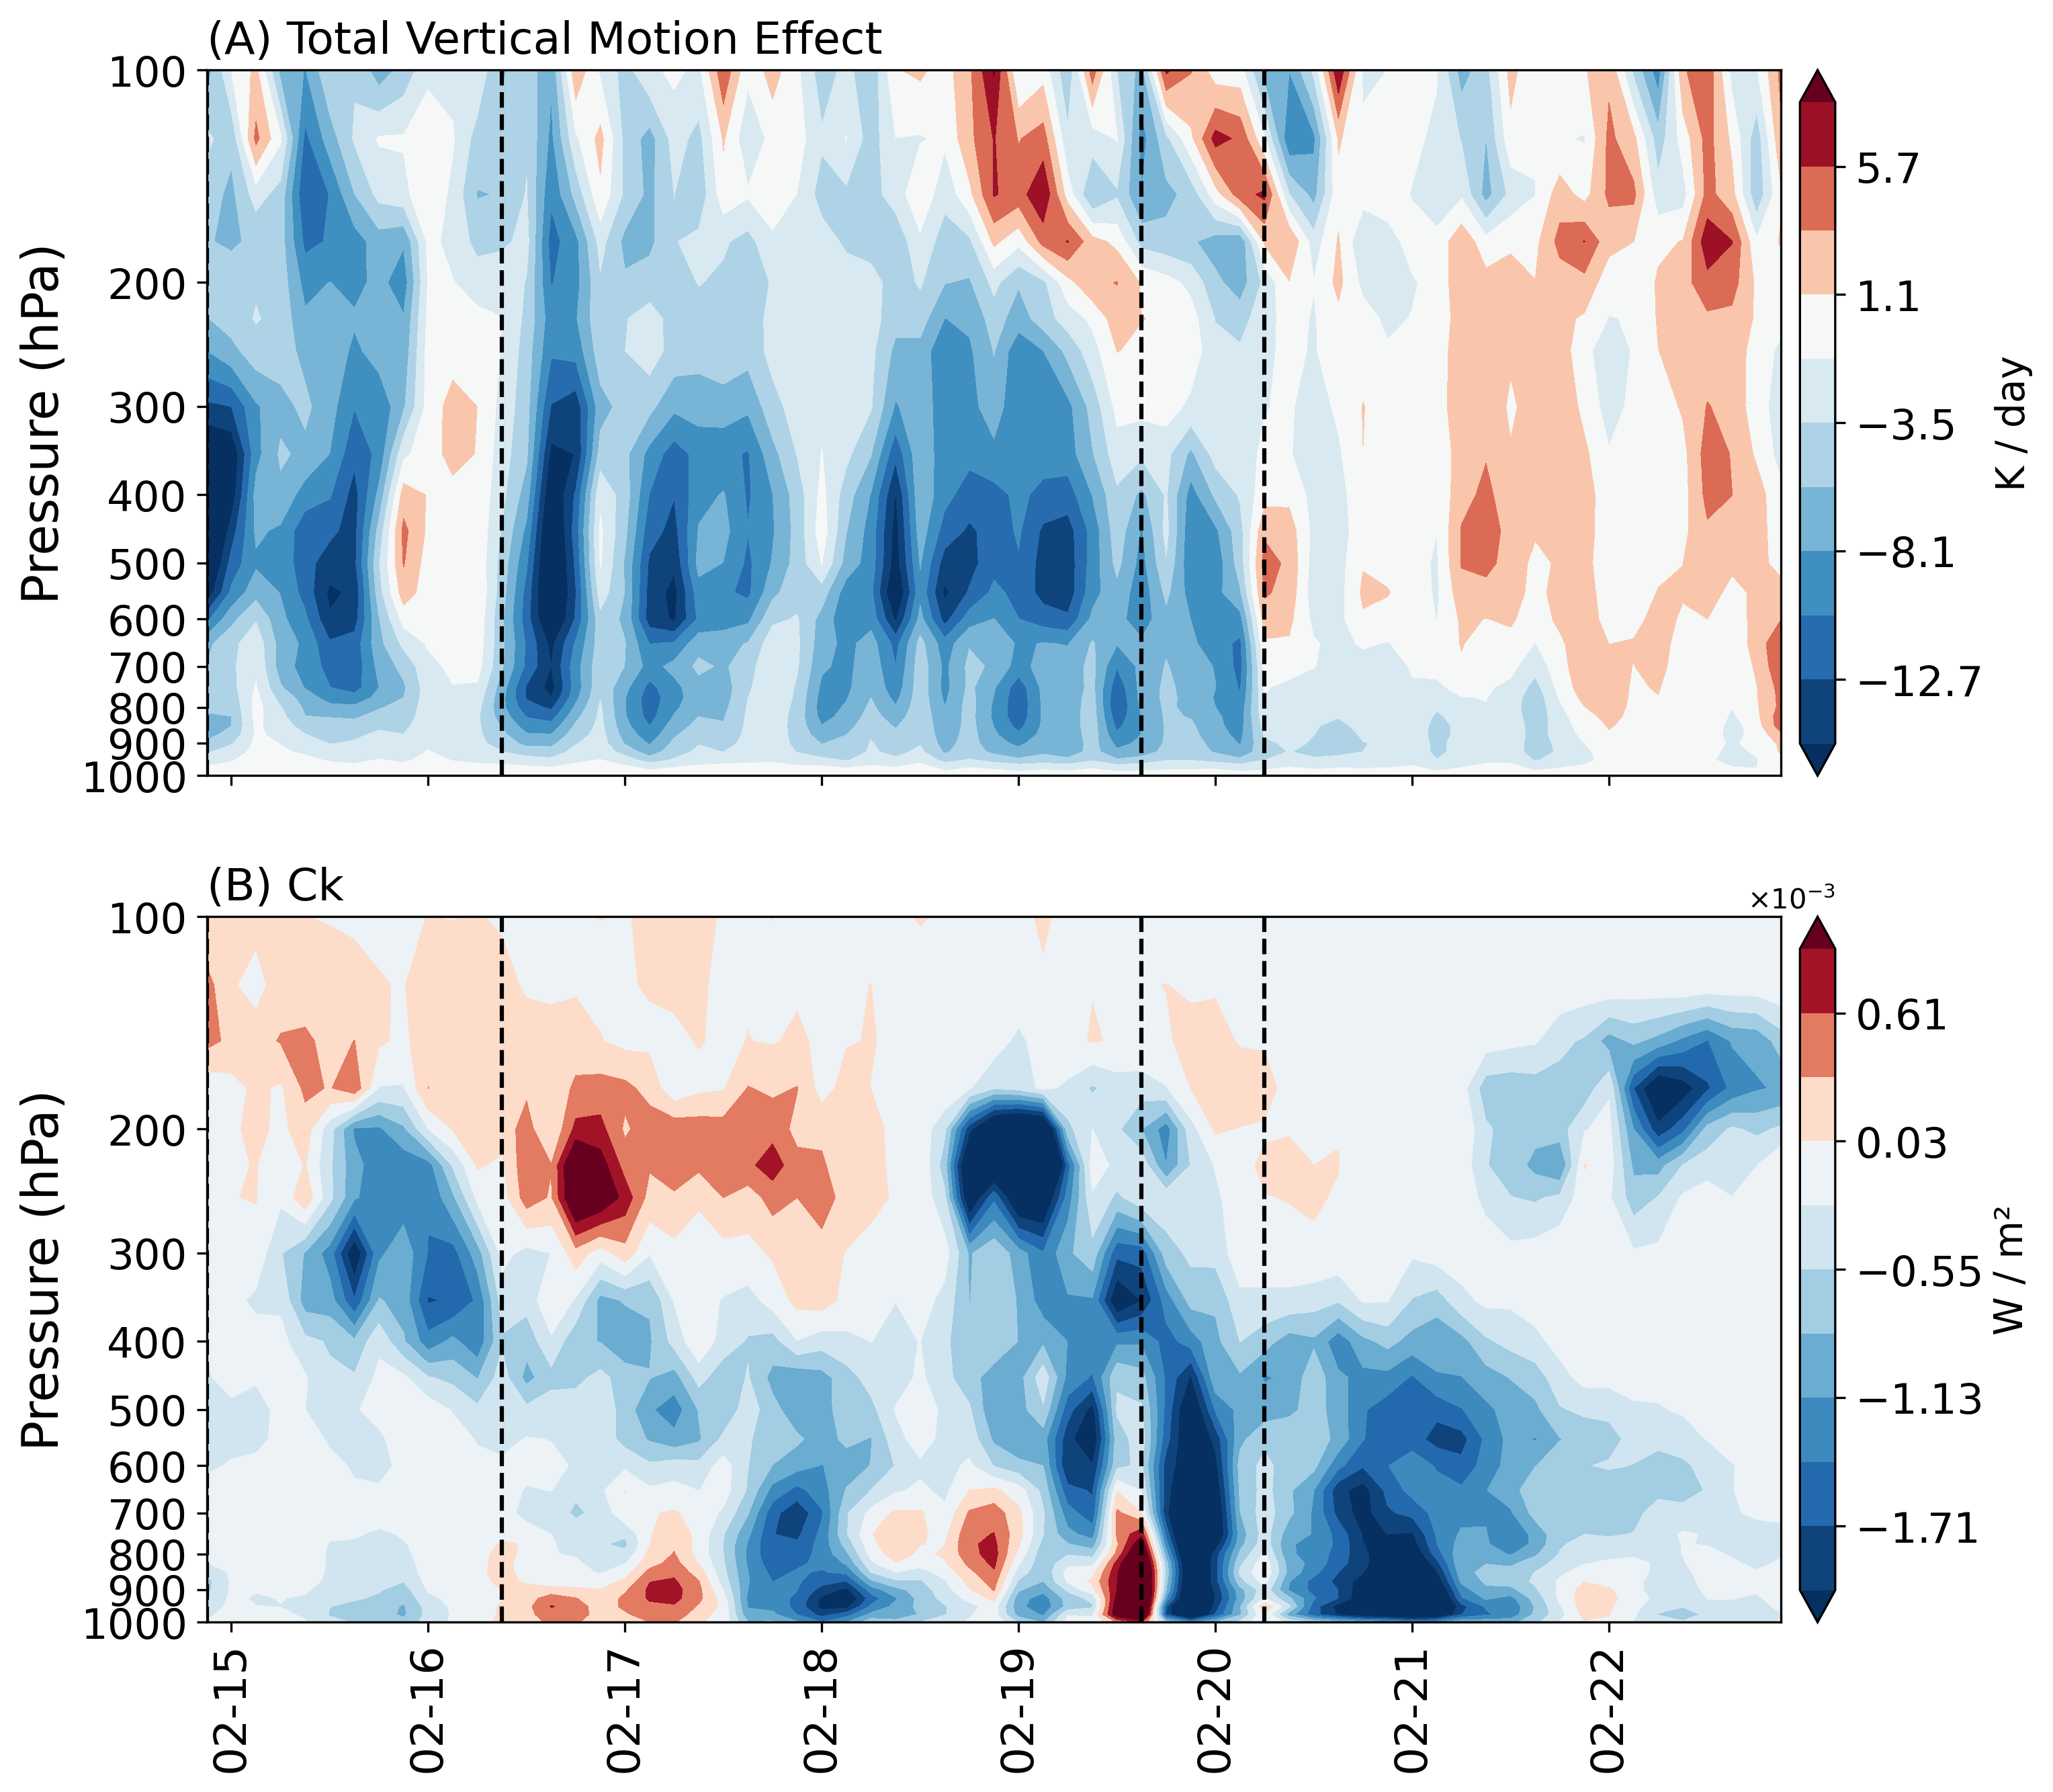
\includegraphics[width=\textwidth]{SigmaOmega_Ck_combined_hov.png}
\caption{(Top) Time–pressure Hovmöller diagram of the total vertical motion effect ($S_p \times \omega$) along the Akará track from February 15 to February 22, 2024, expressed in K~day$^{-1}$. Shading represents adiabatic cooling (blue) and warming (red) induced by vertical motion, with negative values indicating cooling due to upward motion and positive values indicating warming due to subsidence. (Bottom) Time–pressure Hovmöller diagram of the barotropic conversion term ($C_K$) along the Akará track, expressed in W~m$^{-2}$. Negative values (blue) indicate energy conversion from zonal kinetic energy ($K_Z$) to eddy kinetic energy ($K_E$), while positive values (red) indicate the reverse process. Dashed vertical lines mark the key phase transitions in the cyclone's lifecycle: incipient to intensification, intensification to mature, and mature to decay.}
\label{fig:SigmaOmega_Ck_combined_hov}
\end{figure}

\subsection{Decay stage}

Akará enters the decay phase still classified as a tropical cyclone, as evidenced by the CPS (Figure \ref{fig:cps}). However, the zonal mean temperature deviation profile shows the emergence of an upper-level cold anomaly (Figure \ref{fig:combined_serie_zonaldeviation}). From approximately 15Z on February 21 onward, this upper-level cold anomaly intensifies and extends into the mid-troposphere, marking the system's subtropical transition. Accordingly, the CPS indicates a shift from a deep to a shallow warm core during this process, as the system moves over relatively cold waters (Figures \ref{fig:Akara_mean_sst_track} and \ref{fig:Akara_mslp_sst_t2m_multiplot}f).

At this stage, both the vorticity and heat budgets show sharp decreases in the magnitude of all terms. The relatively modest values of FD, ZD, $F_{\zeta}$, and horizontal vorticity advection reflect their previously high magnitudes near the mature phase, which gradually diminish over time. Meanwhile, the system's energy cycle highlights a significant environmental shift, with the conversion terms $C_Z$, $C_A$, and $C_E$ changing sign (Figure \ref{fig:lec}d). Additionally, there are sharp increases in $K_Z$ imports, while the $A_E$ flux across the boundaries also becomes positive. These changes indicate that the decaying system is approaching a weak baroclinic region associated with an upper-level trough at higher latitudes (Figure \ref{fig:Akara_wind_speed_z500_composition}f). Initially, barotropic conversions remain high, particularly up to 600 hPa, but as the system moves closer to the trough, these conversions shift to upper levels.

These atmospheric changes, combined with the system's displacement over relatively cold waters, result in a decrease in convective activity. Consequently, convection near the cyclone center loses its organized structure, and cloud tops become relatively warmer (Figure \ref{fig:ch13}). Notably, a stratospheric incursion occurs at the onset of the decay phase (Figure \ref{fig:SigmaOmega_Ck_combined_hov}). However, without sufficient low-level forcing, this incursion is insufficient to sustain convective activity.


\section{Discussion and Concluding Remarks}


Cyclone Akará originated in a post-frontal, weak baroclinic environment with low vertical wind shear and warm SSTs. During its genesis, SSTs exceeded the $26.5^{\circ}\text{C}$ threshold, typically considered necessary for tropical cyclone development \citep{gray1968global,emanuel1986air}. Although the initial convective activity was linked to the remaining frontal system, the thermal contrast between the cold post-frontal lower troposphere and warm SSTs fueled sensible and latent heat fluxes, which, in turn, sustained Akará's convective activity. Furthermore, a mid-upper tropospheric cutoff low coupled with the surface vortex during this stage, resulting in a subtropical genesis characterized by a weak symmetric warm core, as indicated by \citet{reboita2024assessment}.

Notably, Akará's genesis as a subtropical cyclone was somewhat distinct compared to other subtropical systems. For instance, it was not associated with a mid-to-upper troposphere blocking pattern, a common feature of subtropical cyclogenesis across various ocean basins \citep{da2019subtropical}. Additionally, the development of Tropical Depression Iba and Hurricane Catarina, the only other documented tropical cyclones in the South Atlantic, was linked to such synoptic conditions \citep{pezza2005first,reboita2021iba}. However, other key ingredients identified by \citet{da2019subtropical}, such as isolation from baroclinic influences, persistent ocean-to-atmosphere heat fluxes, and low environmental vertical wind shear, were present during Akará's initial stages. Moreover, the initial energetics of the system — characterized by contributions to eddy kinetic energy from both barotropic and baroclinic chains — align with findings for other subtropical and hybrid systems \citep{michaelides1987limited,dias2013synoptic,pezza2014large,cavicchia2018energetics}.

The system's intensification phase was marked by increased near-surface mass convergence and upper-level mass divergence, which favored upward motion and enhanced convective activity. This occurred as the system moved into a region with SSTs above $28^{\circ}\text{C}$. The further reduction in vertical wind shear supported the organization of convection into a spiral pattern, with Akará developing a barotropic structure. The environment also transitioned to being less baroclinic and more barotropic, with mid to low-level barotropic conversions playing a key role in fueling the system's development.

During the intensification phase, Akará underwent tropical transition, evolving to exhibit a deep warm core. This transition coincided with an increased thermal contrast between the ocean and atmosphere, which further enhanced near-surface heat fluxes, reducing stability and promoting convective activity. While convective processes undoubtedly contributed to heating the atmospheric column, we propose that stratospheric air intrusions were critical to the tropospheric heating that characterized Akará's tropical transition. These intrusions intensified the mid-upper-level cyclonic circulation, providing dynamical support for convective activity in a post-frontal barotropic environment. The dynamical origins of these intrusions warrant further investigation, and we recommend future studies employing numerical simulations to assess their relative importance for Akará's tropical transition. Moreover, the role of stratosphere-troposphere interactions during Catarina's tropical transition has not yet been explored. Determining whether such interactions are fundamental to tropical transitions in the South Atlantic is crucial for improving our understanding and forecasting of these rare events.

The cyclone reached its mature phase with warm anomalies throughout the troposphere, intensifying its deep warm-core structure. The system's cloudiness became fully detached from the preceding frontal structure and exhibited an eye, as reported by the Brazilian Navy \citep{marinha2024}. However, during this phase, convective activity decreased compared to earlier stages as the system moved over colder waters (below $25^{\circ}\text{C}$), despite increased near-surface mass convergence. Stratospheric air intrusions persisted during the mature phase and may have contributed to maintaining the observed warm-core structure, compensating for the reduced latent heat release. The signature of these intrusions is visible in the total vertical motion effect but is less evident in the heat budget due to period averaging.

Although barotropic conversions increased significantly during the mature phase, high surface friction and the export of eddy kinetic energy acted as brakes on further development. Notably, barotropic conversions were intense from the surface to the mid-troposphere, while the baroclinic chain remained inactive, reflecting the cyclone's barotropic environment. This transition of barotropic conversions, shifting from the upper troposphere to the mid-to-low levels, was also observed during Catarina's tropical transition \citep{veiga2008analysis}. While studies analyzing the evolution of barotropic instability profiles in tropical cyclones remain scarce, numerical and observational evidence indicates that low-level barotropic instability is a primary mechanism associated with initial vortex formation in tropical disturbances within the Intertropical Convergence Zone (ITCZ), which often serve as precursors to tropical cyclones \citep{ferreira1997barotropic,yokota2012tropical,yokota2015tropical,bembenek2021influence}. Beyond the ITCZ, African Easterly Waves, which are precursors to tropical cyclones in the Northern Atlantic, are also strongly linked to mid-to-low-level barotropic instability \citep{burpee1972origin,rennick1976generation,molinari1997potential,reed1977structure,wu2012african}. These connections highlight the critical role of barotropic processes in tropical cyclone genesis. Further research is necessary to investigate the role of barotropic instability and its vertical distribution in tropical cyclones, particularly in regions like the South Atlantic where these systems are rare. A more comprehensive understanding of these dynamics could improve our knowledge of the mechanisms driving vortex formation and development, ultimately enhancing predictions of tropical cyclogenesis and evolution in underexplored basins.

Following its mature phase, Akará experienced further reductions in convective activity, as the system's cloudiness lost its organizational structure. This decay phase was marked by sharp decreases in both heat and vorticity budget terms, as well as environmental changes near the cyclone center, with the system approaching a baroclinic zone. Barotropic conversions diminished during this phase, shifting from peaking near the surface to occurring at upper levels. During its decay, Akará underwent subtropical transition, marked by cooling in the mid-to-upper troposphere, movement over colder waters (below $23^{\circ}\text{C}$), and displacement into a colder atmospheric region at lower latitudes (below $32^{\circ}\text{S}$).

In conclusion, this study provides valuable insights into the dynamical, thermodynamical and energetic features of a rare tropical transition event in the South Atlantic, as suggested by \citet{reboita2024assessment}. The analysis of Akará's life cycle phases proved valuable for understanding the dynamic, thermodynamic, and environmental shifts during its development, complementing the thermal structure analysis that highlighted the cyclone's transition from a subtropical to a tropical system. Future research focusing on similar tropical transition events could enhance our understanding of the mechanisms underlying these processes, particularly in the South Atlantic, where such occurrences are rare. Comparative studies with other tropical transitions, such as those of Hurricane Catarina and Tropical Depression Iba, or with subtropical cyclones that did not undergo tropical transition, could offer valuable perspectives on the conditions and factors influencing these systems. Such research would also contribute to improved forecasting and risk assessment for similar events in the future.


\backmatter

% \bmhead{Supplementary information}

% If your article has accompanying supplementary file/s please state so here. 

% Authors reporting data from electrophoretic gels and blots should supply the full unprocessed scans for key as part of their Supplementary information. This may be requested by the editorial team/s if it is missing.

% Please refer to Journal-level guidance for any specific requirements.

%TC:ignore
\section*{Declarations}

\subsection*{Funding}

This study was partly financed by the Coordenação de Aperfeiçoamento de Pessoal de Nível Superior – Brasil (CAPES) under Finance Code 001.

\subsection*{Competing interests}

The authors have no relevant financial or non-financial interests to disclose.

\subsection*{Data Availability}

The data supporting the findings of this study, including the results of the Lorenz Energy Cycle and the heat and vorticity budget analyses, are openly available in the following repositories. The complete diagnostics and plotting scripts for Cyclone Akará are available at: \url{https://github.com/Victorrani/Cyclone_Analysis/tree/main/Akara}. The LorenzCycleToolkit, used to compute the Lorenz Energy Cycle, is available at: \url{https://github.com/daniloceano/LorenzCycleToolkit}. The ATMOS-BUD framework, used for calculating heat and vorticity budgets, is available at: \url{https://github.com/daniloceano/ATMOS-BUD}. All datasets and scripts are publicly accessible and can be used to reproduce the analyses presented in this manuscript.

\subsection*{Author contributions}

\begin{itemize} \item \textbf{Danilo Couto de Souza:} Conceptualization, Methodology, Software, Formal Analysis, Investigation, Writing - Original Draft, Writing - Review \& Editing. \item \textbf{Victor Antunes Ranieri:} Formal Analysis, Data Curation, Investigation.  \item \textbf{Pedro Leite da Silva Dias:} Supervision, Writing - Review \& Editing, Methodology, Analysis Support. \item \textbf{Andrés Rodríguez Flores:} Formal Analysis, Data Curation, Investigation. \item \textbf{Ricardo de Camargo:} Supervision, Writing - Review \& Editing, Analysis Support. \end{itemize}

\bibliography{sn-bibliography}% common bib file
%% if required, the content of .bbl file can be included here once bbl is generated
%%\input sn-article.bbl


\end{document}
